\documentclass[12pt]{article}
\usepackage{graphicx} % Required for inserting images
\usepackage{float}
\usepackage{geometry}




\graphicspath{ {/home/gonzalopc/Documentos/programas_mios/TFM_AFI_2025/TFM_AFI_2025/mynotes/images/} }

\setlength{\parskip}{4mm}
\textwidth 15cm
\leftmargin 2cm
\rightmargin 1cm
\setlength{\baselineskip}{18pt}

\title{Transporte marítimo e incautación de droga}
\author{Gonzalo Lopez Segovia}
\date{December 2024}

% Keywords command
\providecommand{\keywords}[1]
{
	\small	
	\textbf{\textit{Keywords---}} #1
}

\geometry{
	a4paper,
	total={170mm,257mm},
	left=20mm,
	top=20mm,
}

%\renewcommand{\baselinesetstretch}{1.25}

\begin{document}
	
	%Incluir Logo AFI en la Portada

	
\Large

\maketitle

\newpage

\section{\label{resumen}Resumen}

\section{\label{abstract}Abstract}


\keywords{Transporte marítimo, Geografía del Transporte, Geografía Marítima, Drogas, Estupefacientes, Narcotráfico, Machine Learning, Análisis de Datos, Clustering}

\newpage
% Añadir indice de contenidos

\section{\label{intro}Introducción}
	El transporte marítimo ha sido, desde la Antigüedad, el eje central del comercio global. Imperios y civilizaciones han dependido de rutas marítimas para el intercambio de bienes, desde las redes comerciales del Mediterráneo hasta las rutas coloniales que unieron continentes en la era moderna. Sin embargo, fue la Revolución Industrial la que transformó radicalmente la logística marítima, con avances avances en la construcción naval y, más recientemente, con la revolución de la contenerización iniciada en 1956 por el Ideal-X en su ruta Newark-Houston \cite[]{}. Este cambio permitió una drástica reducción en los tiempos y costos de carga y descarga, consolidando el transporte de contenedores como el estándar del comercio global. Hoy en día, la mayor parte del comercio internacional depende de esta infraestructura, con puertos como Los Ángeles, Shanghái y Rotterdam actuando como nodos críticos de la economía mundial.
	
	No obstante, la misma eficiencia y globalización que han impulsado el comercio legal han facilitado también el tráfico de productos ilegales, especialmente drogas. Los puertos marítimos, debido a su alto volumen de carga y complejidad logística, representan un punto vulnerable para el contrabando de sustancias ilícitas. Aprovechando las rutas comerciales establecidas y las infraestructuras portuarias, es posible ocultar cargamentos de drogas entre mercancías legítimas, desafiando los sistemas de inspección y control aduanero. Este fenómeno no es reciente: desde las Guerras del Opio en el siglo XIX hasta la actual crisis de opiáceos, el narcotráfico ha estado intrínsecamente ligado a las dinámicas del comercio global.
	
	Estados Unidos, como principal mercado de consumo, y China, como fuente de precursores químicos, ejemplifican la interconexión entre el comercio legal e ilegal en la actualidad. Los flujos comerciales reflejan no sólo la globalización económica, sino también la propagación de bienes de consumo ilícitos a través de las mismas infraestructuras que sustentan el comercio mundial. En este contexto, el estudio del tráfico marítimo y la incautación de droga en puertos se vuelve crucial para comprender los patrones delictivos y fortalecer las estrategias de detección y control.
	
	Este trabajo explorará la relación entre el comercio marítimo y el tráfico de drogas, analizando datos sobre el movimiento de contenedores y las incautaciones realizadas en los principales puertos de EE.UU. a partir de registros oficiales del CBP \cite{}. A través de un enfoque basado en datos, se intentará identificar, si fuera posible, patrones geográficos, de tendencias temporales o si existiese la correlación entre el volumen de contenedores manejados por cada puertoy la cantidad de incautaciones reportadas por sus correspondientes "Field Offices" del CBP.
	
	El objetivo de este trabajo es intentar aportar una visión cuantitativa sobre cómo el tráfico marítimo y las operaciones de control en los puertos de EE.UU. interactúan en el contexto del narcotráfico, pudiendo proporcionar información valiosa para mejorar las estrategias de detección y prevención.
	
	

	\subsection{\label{antecedentes}Antecedentes}
	Importancia del transporte marítimo en el comercio global:
	\begin{description}
		\item[-] Según el documento de la OECD (An Ocean of Data) más del 80\% del comercio global en volumen y el 70\% en valor se transporta por vía marítima \cite[]{}.
		\item[-] Los puertos son nodos críticos para la economía mundial, funcionando como infraestructuras de interconexión entre lo local y lo global.
		\item[-] Las nuevas tecnologías, como los sistemas AIS, han permitido un mejor rendimiento de la actividad portuaria y del tráfico comercial, lo que facilita el análisis de patrones comerciales y posibles interrupciones.
		\item[-] En 2019, el volumen total de mercancías transportadas por mar superó los 11.000 millones de toneladas métricas. \cite[]{https://www.cidob.org/publicaciones/infografias-transporte-maritimo-factor-clave-del-comercio-global?utm_source=chatgpt.com}
	\end{description}
	
	Relación con el tráfico de drogas:
	\begin{description}
		\item[-] A partir del trabajo realizado por Coufal para la Universidad de Amsterdam \cite[]{} para los puertos de Roterdam y Amberes se intentará realizar un análisis para los puertos de EE.UU.
		\item[-] La enorme cantidad de contenedores que llegan diariamente dificulta la detección de cargamentos ilícitos, lo que convierte a estos puertos en objetivos estratégicos para el crimer organizado.
	\end{description}

	En definitiva, las investigaciones previas en los que se basa este tabajo sirven para mostrar como el crecimiento del comercio marítimo junto con la voluminosa gestión de cargamento dificulta la detección de estupefacientes y, a su vez, facilita su introducción en mercados de alto consumo a través de los mismos.
	
	\subsection{\label{motivacion}Motivación del proyecto}
	% Descripción del problema
	El origen de este proyecto se basa principalmente en el interés de aplicar los conocimientos sobre la geografía humana a nivel del comercio internacional. Esto junto con informaciones de interés relacionado con ciertas actividades ilícitas que se dan en zonas portuarias, dio paso a intentar averiguar si se podía estimar la cantidad de droga que entraba en un puerto cualquiera a partir del trasiego de contenedores en un puerto comercial. Pese a que en un principio se intentó realizar para la vía comercial del Pacífico exclusivamente y basándose en el flujo de barcos cargueros entre estas regiones, las dificultades a la hora de obtener datos de fuentes privadas (necesidad de obtención una licencia para explotar los datos), hizo desde muy pronto bajar las expectativas y reformular el punto de partida.
	
	Las fuentes privadas orientadas a la explotación de los datos a nivel empresarial, facilitan un enfoque para cualquiera de estas empresas relacionadas con el comercio, los procesos logístico o la especulación financiera. Los datos abiertos, con un enfoque de más información transparente sobre resultados de administraciones, podrían en parte suplir las carencias de no poder acceder a las fuentes privadas. Es por ello que el problema se reorienta desde un punto de vista del transporte de mercancías por flujo de barcos al del trasiego de contenedores gestionado por la autoridad portuaria pertinente.
	
	Y como se venía diciendo, la motivación original de este proyecto era ir un paso más allá, intentar averiguar el flujo de entrada de droga a partir de datos de incautaciones. Sin embargo, como se verá a lo largo de este trabajo, quedará demostrado que con los datos aportados no es suficiente para predecir. Al ceñirse a actividades de éxito de las agencias de aduanas se encontrarán una serie de impedimentos:
	
	\begin{description}
		\item[1.] Pese a centrarse en actividades en puertos y fronteras, la cantidad estimada de contenedores que se investigan son apenas un 5 por ciento de los contenedores totales que pasan a diario \cite[]{}.
		\item[2.] No solo eso, los hubs portuarios se sitúan en las conocidas como ciudades globales \cite{} de gran importancia económica, con gran intermodalidad entre distintos medios de transporte y capaz de conectar vías de alta capacidad, por lo que el nivel de alcance se hace demasiado extenso para poder incautar toda la droga que entra.
		\item[3.] La forma de abordar el problema relacionado con el narcotráfico a distintos niveles administrativos, junto con la legalidad de ciertas sustancias, hace que el problema no solo dependa de la cantidad que llega (la demanda) sino de la aproximación a nivel político: si se es más laxo con cierta sustancia o, por el contrario, más estricto.
	\end{description}
	
	Esto, como se verá más adelante \ref{Diseño}, impedirá realizar un buen análisis a partir de los datos tratados.
	
	Gran parte del origen del trabajo surge a partir del interés por la Geografía Económica y del Transporte. Trabajos como el publicado por Jean-Paul Rodrigue en \cite[]{} ha servido, a pesar de todo, como acicate para aunar y profundizar conocimientos en este campo y aplicarlo a una temática sensible como es el tráfico de estupefacientes. A partir de los datos recopilados, se intentó que de algún modo u otro se pudiera si no responder, al menos plantear de forma clara la siguiente conjetura: Si conocemos la actividad económica en un puerto -entendida como trasiego de contenedores-, ¿sería posible, solo con esa información, estimar el volumen de incautación de droga para ese mismo puerto? Se deja la ventana abierta a que se trate de una droga en particular, que sea el número de redadas o que sea la cantidad (kilogramos o libras) y que sea para un puerto en exclusiva o si se pudiere generalizar a varios puertos.\
	 
	\subsection{Objetivos}
	De acuerdo con los expuesto en la sección "Motivación del proyecto", este trabajo se va a encargar de:
	
	\begin{description}
		\item[1] Agrupar puertos en regiones geográficas y metropolitanas próximas denominadas "hubs portuarios" a partir de señales de comunicaciones enviadas desde barcos próximos.
		\item[2] Mostrar el comportamiento de distintos puertos con respecto al volumen de droga incautada por tipo de droga.
		\item[3] Estudiar si el comportamiento puede ser caracterizado por factores periódicos en forma de serie temporal para un intervalo de 75 meses (6 años y 1 trimestre).
		\item[4] Determinar si a partir de la actividad en un puerto comercial, dado volumen de carga y descarga en ese puerto, se podría estimar la cantidad de droga incautada en ese mismo puerto.
	\end{description}

	% Conocimientos: Estadística Descriptiva, Series Temporales, Clustering, Visualización, Ensemble Learning.

	\subsection{Enfoque y Metodología general}
	Para la realización de este proyecto, se necesita tener conocimientos sobre estadística descriptiva, series temporales, clustering, visualización de datos, y algoritmos de aprendizaje automático (Machine Learning), especialmente en Árboles de decisión y ensemble learning.

	\subsection{Estructura del Documento}
	Este trabajo se divide en: una introducción donde se exponen los antecedentes, motivaciones y objetivos; una sección sobre el Estado del Arte tanto a nivel de técnicas y algoritmos de Machine Learning como conocimientos relacionados con el objetivo del problema (relacionar Geografía del Transporte con las dinámicas del narcotráfico); otra sección sobre la metodología empleada en la que se detalla largo y tendido tanto el tratamiento de los datos como planteamiento del modelo que emularía el problema; otra sección "Diseño del Modelo" con los algoritmos aplicados, la implementación y la evaluación del rendimiento. Para terminar con las secciones sobre la interpretación (y visualización de los resultados) y conclusiones y trabajos futuros.

\newpage

\section{Estado del arte}
Al faltar datos de flujos y vías marítimas, no es trivial hallar la red o grafo mundial de conexiones portuarias.

	\subsection{Literatura sobre el problema}
	Para el desarrollo del modelo se ha intentado que, a nivel de técnicas de Machine Learning, las soluciones propuestas estuviesen integradas en librerías de python como scikit-learn o prophet, para facilitar y acelerar su implementación. También se ha leído algo de bibliografía relacionada con el alcance del problema. Así pues, libros y estudios sobre la geografía del transporte como informes sobre las dinámicas del narcotráfico a nivel global han servido para intentar guiar el trabajo realizado. 
	
		\subsubsection{Estudio de la Geografía del Transporte.}
		% Los puertos más transitados de Estados Unidos de América.
		
		
		
		\subsubsection{Estudio sobre dinámicas del narcotráfico}
		% https://upcommons.upc.edu/bitstream/handle/2117/392133/181021_TFG_final.pdf?sequence=2
		% Cities, Ports, and Drug Trafficking By Tomas Coufal


	\subsection{Conocimiento de técnicas de Machine Learning}
	El análisis del tráfico y la detección de actividades ilícitas, como el tráfico de drogas, han sido históricamente abordados mediante métodos tradicionales basados en reglas, estadísticas descriptivas y técnicas de minería de datos convencionales \cite{}. Los enfoques efectuados entonces presentaban determinadas carencias como son el alto grado de supervisión humana, la dificultad para detectar patrones ocultos y su escalabilidad limitada.
	Por contra, los enfoques basados en técnicas y conocimientos de Machine Learning y Data Science ofrecen una mayor capacidad de análisis, permitiendo encontrar patrones complejos, anticiparse mediante el análisis predictivo o detectar anomalías entre otros.
	
	En estudios previos sobre el tráfico marítimo y la detección de actividades ilícitas, se han utilizado diversos modelos y técnicas de Machine Learning entre los cuales, algunos de ellos serán utilizados a lo largo de este trabajo.
	
		\subsubsection{Algoritmos de Predicción}
		En el contexto de este estudio, se van a emplear algoritmos de Machine Learning enfocados en la predicción de valores numéricos a partir de datos históricos. Puesto que en este caso, uno de los propósitos es resolver un problema de regresión, se ha decidido realizar pruebas con modelos basados en árboles de decisión y técnicas, tanto de boosting como de bagging. Los algoritmos considerados candidatos vendrían a ser:
		
		\begin{description}
			\item Árboles de Decisión.
			\item Regresión Lineal.
			\item Adaboost: técnica de boosting a partir de árboles muy sencillos (modelos débiles) asignando mayor peso a los datos peor predichos.
			\item Bagging: conjunto de múltiples árboles compuesto por el subconjunto aleatorio de variables y observaciones.
			\item GradientBoost: Algoritmo de boosting con librería de python propia. Su función de pérdida es diferenciable.
		\end{description}


		\subsubsection{\label{prophet}Series temporales con Prophet}
		Puesto que uno de los objetivos originales del problema era, en caso de que fuera posible, a partir de una serie temporal sobre la llegada de cargamentos, hallar la cantidad de droga incautada (con independencia del tipo). Sin embargo, quizá fuese la falta de horizonte temporal, o ciertas características que pudieran condicionarla como una serie temporal (estacionaria en media, con varianza constante...) dificultó la buena realización de un problema de esta índole. Sin embargo, en algún caso que si se demostró factible se hizo uso de la librería prophet de Meta para la resolución de series temporales.
		
		Para una serie temporal hay que considerar su tendencia a nivel general, si tienen comportamientos estacionales y el resto que no pudiere ser caracterizado, identificarlo como ruido blanco gaussiano (el residuo) \cite{}.
		
		% Incluir alguna imagen de ejemplo de como tratar una serie temporal

		\subsubsection{\label{clustering}Técnicas de clustering}
	%	 Incluir Vectorial K-Means (*)\
		Dada la gran disparidad entre el número de puertos y el número de oficinas aduaneras del CBP, se estimó necesario la agrupación de los primeros en "hubs portuarios". Para ello se barajaron distintas técnicas de clustering para poder agrupar las señales emitidas por aquellos barcos de tipo carguero (cargo ship) que se encontrasen de algún modo atracados a lo largo de una serie de días de septiembre de 2024. A partir de las señales de los barcos, se aplicó un algoritmo K-Means tradicional para hallar aquellos puntos cercanos al litoral que mejor agrupasen barcos (y, en definitiva, puertos) cercanos entre sí.
		
		Para este problema, se utilizó 'silhouette', en detrimento de otras opciones. También se estimó el uso de de alternativas como K-Means Vectorial \cite[]{https://arxiv.org/abs/1208.5801}, pero debido a su alcance más de nicho (no implementado en scikit-learn o cualquier otra gran librería de Python) frenó sus posibilidades de implementación, junto con la poca claridad del objetivo final del problema por aquel entonces. Otros algoritmos que se tuvieron en cuenta fueron PAM y los de tipo jerárquicos, pero para las necesidades requeridas bastó con K-Means aplicado sobre las variables de latitud y longitud.	
		
	\subsection{Justificación de las herramientas y tecnologías elegidas}
	Python, pandas, scikit-learn desarrollos con Google Colab y en VisualStudio en función de si se requería una gran capacidad de cálculo. Debido a los cambios constantes en los planteamientos y objetivos del problema a causa de las dificultades inherentes a la captura e integración de datos, se fueron reinstanciando los distintos bloques, siendo algunas partes originales del problema desestimadas. Sin embargo, se decidió rescatar el problema de clustering de puertos para generar el hub portuario, aunque como se menciona en la subsección \ref{clustering} se extrajeron seis hubs portuarios lo suficientemente representativos para después continuar con el desarrollo del problema.
	
	%Técnicas de clustering para cita en parrafo anterior
\newpage
	
\section{Metodología empleada}	
Este trabajo busca identificar patrones, correlaciones y tendencias entre el volumen de cargamento trasegado en una serie determinada de puertos de EE.UU. y la cantidad de droga incautada por las secciones adyacentes del servicio de aduanas (CBP). Para ello a continuación se detalla la metodología que se ha seguido para implementar una serie de técnicas de análisis de datos y Machine Learning.

	\subsection{Descripción del conjunto de datos utilizado}
	Para la puesta a punto del conjunto de datos a tratar, primero hubo que implementar un desarrollo de integración de los mismos provenientes de distintas fuentes.
	Para ello, hubo que conseguir un compromiso entre aquellos datos obtenidos del transporte de mercancías en puertos marítimos con los datos oficiales sobre incautaciones. La clave para ello estuvo en estandarizar el intervalo y el nivel de detalle en el eje temporal (meses para los últimos seis años fiscales en EE UU) y en el nivel geográfico.
	
		\subsubsection{\label{data origin}Origen de los datos}
		%Primera aproximación al problema
		Originalmente, el objetivo del trabajo buscaba relacionar el comercio global y sus flujos regionales con el tráfico de drogas. Debido a las complejidades a la hora de acceder a estos datos y que estos dependen de agencias privadas (bajo licencia), se replanteó el problema de tal modo que se trabajasen sobre puertos destino en Estados Unidos (datos abiertos) y no sobre un modelo de grafos basado en las rutas marítimas de transporte. La ventaja de los datos provistos por Estados Unidos (ya sea a nivel federal, nivel estatal o local) es que éstos suelen ser de buena calidad.
		
		\underline{Fuentes, Bases de Datos, Informes}\\
		Los datos de transporte de contenedores se obtuvieron de las distintas páginas webs informativas de cada autoridad portuaria. Accediendo a las secciones de informes estadísticos se pudieron obtener datos a nivel mensual sobre carga y descarga de contenedores, así como exportaciones e importaciones. Todos aquellos puertos de EE UU que proveyeron esta información fueron considerados objeto de estudio. Por otro lado, los datos referidos a incautaciones de drogas se obtuvieron los informes estadísticos de incautación de droga provistos por la CBP (Agencia de aduanas de Estados Unidos) para las distintas oficinas regionales a nivel mensual para los años fiscales 2019 a 2024.
		
		% Imagen web CBP
		
		Una vez se localizaron las fuentes y los datos de interés, se procedió a su descarga. La construcción del dataset de entrada se trató de un problema de integración de datos. Se usó tanto la fecha (en formato "Año-mes") como la región geográfica como clave primaria para unir los datos de trasiego de contenedores en un puerto como de incautaciones de drogas para oficinas del CBP asignadas para su hub portuario correspondiente. Ya que a nivel temporal, el nivel de detalle que se pudo conseguir fue a nivel mensual, se obtuvieron de partida setenta y cinco meses de observaciones (equivalentes a seis años más un trimestre debido a que los años fiscales en Estados Unidos comienzan el 1 de octubre del año natural anterior).
		
		Dado que el CBP se trata de una agencia federal de Estados Unidos,se evitó el inconveniente que pudiera acarrear si cada estado tuviese su agencia propia y no existiese una estandarización de los procedimientos y oficinas. Todos aquellos puertos que ofrecieron datos de calidad en relación a operaciones sobre contenedores (total de TEUs, Importaciones Totales, Exportaciones Totales, Contenedores Vacíos y Contenedores Llenos) y que resultasen de interés para el trabajo, fueron incluidos.
		
		\underline{Detección de hubs portuarios}\\ %: Clustering.
		Como se mencionó en la sub-sección \ref{clustering}, para simplificar el número de puertos y poder asignarlos a las oficinas del control de aduanas de Estados Unidos, se procedió a usar técnicas de Clustering (K-Means). Esto se hizo para poder estimar en qué regiones geográficas se podían agrupar aquellos puertos que fueran cercanos geográficamente entre sí. 
		
		\begin{figure}[H]
			\caption{\label{map_cluster_1} Señales AIS de barcos recopilados por el NOAA}
			\centering
			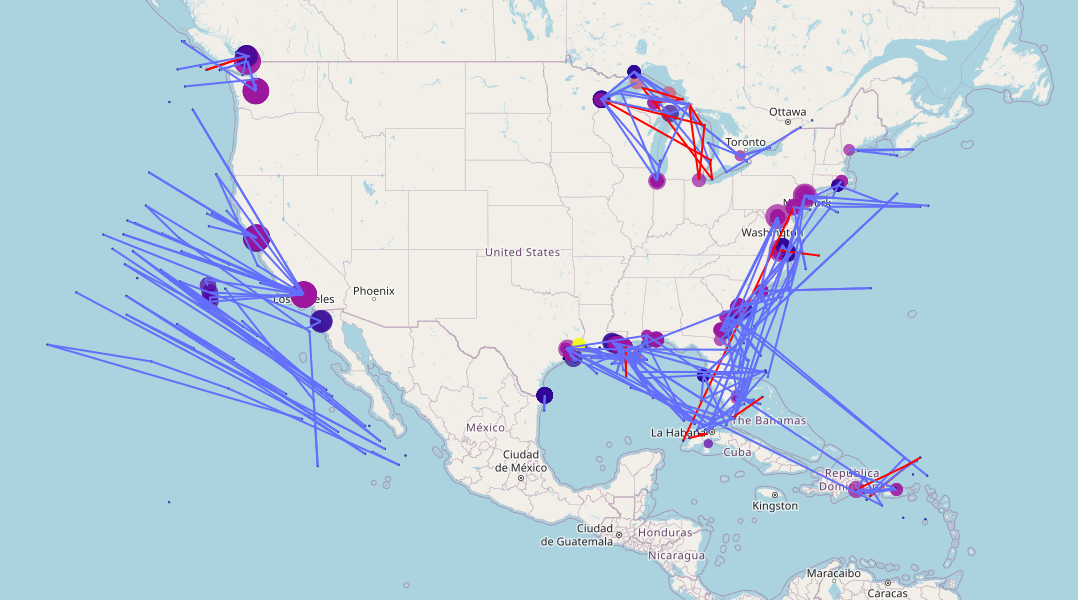
\includegraphics[width=0.5\textwidth]{map_cluster_1.png}
		\end{figure}
		
		Originalmente, se estimó implementar una versión para el algoritmo k-Means vectorial \cite{}. En la imagen \ref{map_cluster_1} se muestra la captura de señales AIS de cada barco cada veinticuatro horas durante un periodo de catorce días en septiembre de 2024. Sin embargo, dadas las complejidades inherentes al algoritmo se decidió probar otras vías.
		
		De una manera mucho más simple, se decidió reciclar los datos obtenidos entonces, para esta vez filtrar qué barcos se encontraban atracados o con el motor parado y cerca de las costas. Según la documentación aportada por el NOAA (agencia federal atmosférica de Estados Unidos), la tabla de datos incluía una variable 'Status' entre los cuales los valores '1' y '5' correspondían con esos casos. En la imagen \ref{map_cluster_2} se muestra un mapa con aquellos barcos con dichos status.
		
		\begin{figure}[H]
			\caption{\label{map_cluster_2} Señales AIS de barcos atracados o con movilidad restringida recopilados por el NOAA}
			\centering
			\hspace*{1cm}
			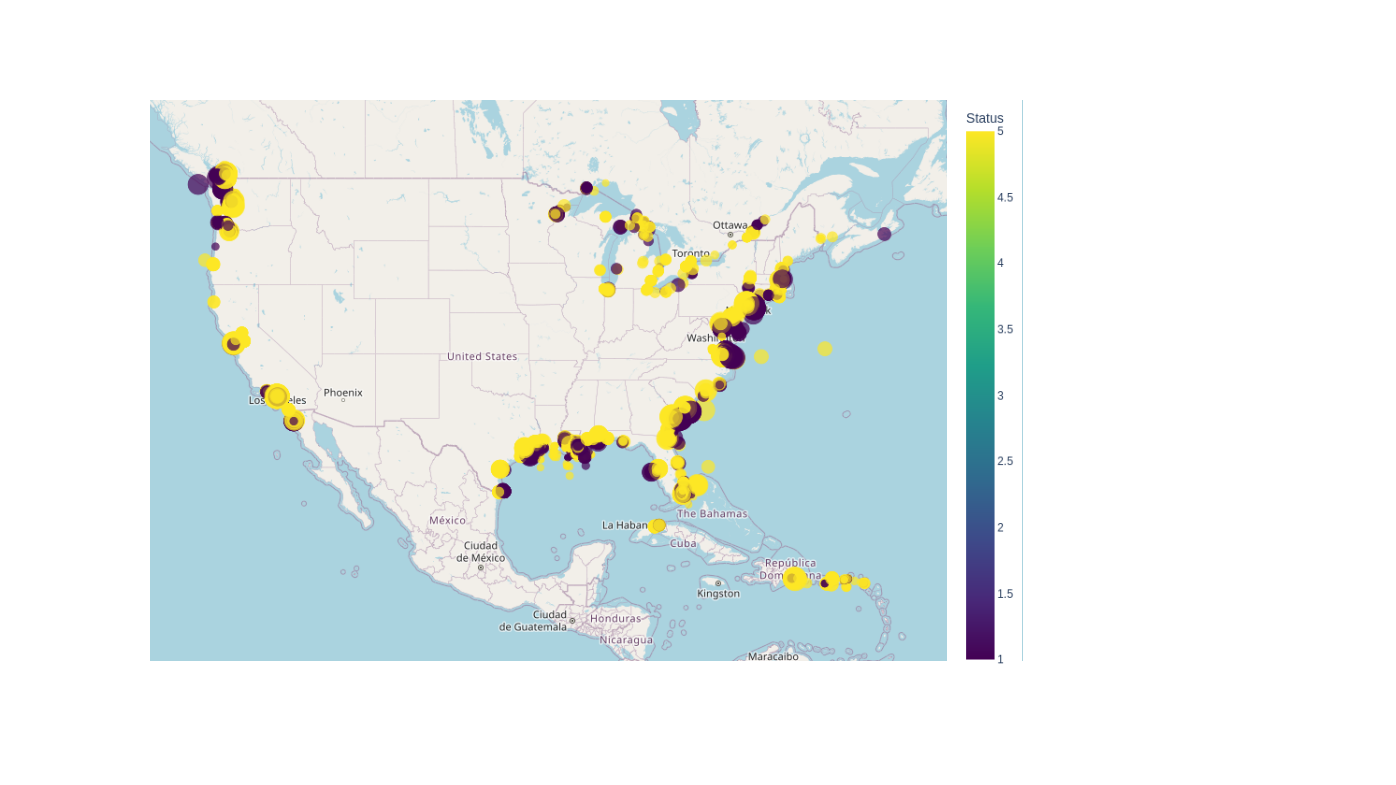
\includegraphics[width=0.8\textwidth]{map_cluster_2.png}
		\end{figure}
	
		Una vez filtrados los barcos con ese status (y con proximidad al litoral), se pudo realizar la agrupación basándose en las variables de coordenadas (latitud y longitud). Usando un k-Means con, originalmente, una treintena clusters, se obtuvieron los potenciales hubs portuarios para considerar dentro del análisis (Véase la imagen \ref{map_cluster_3})
		
		\begin{figure}[H]
			\caption{\label{map_cluster_3} Señales AIS de barcos atracados o con movilidad restringida recopilados por el NOAA}
			\centering
			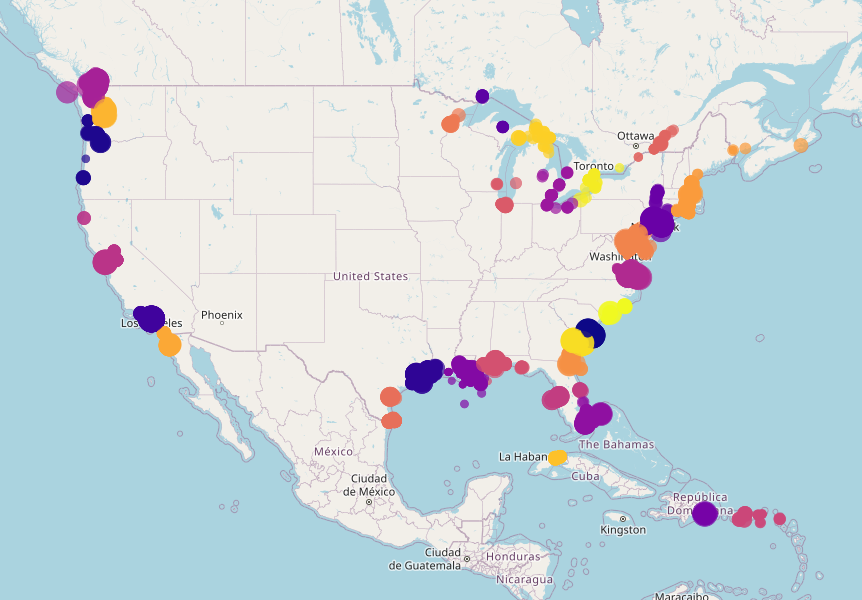
\includegraphics[width=0.5\textwidth]{map_cluster_3.png}
		\end{figure}
		
		 El resultado fue la asignación de coordenadas esféricas a partir de las señales emitidas por los barcos mercantes y detectadas por la agencia meteorológica de EE UU (NOAA, por sus siglas) durante quince días del mes de septiembre de 2024. Estas coordenadas sirvieron para estimar de forma aproximada barcos atracados en puertos próximos entre sí y, en último término, asignarlas a oficinas del CBP. Gracias al conocimiento geográfico de Estados Unidos, no fue demasiado complicado asignar los hubs portuarios a las agencias aduaneras.
		 
		 Debido a las complejidades y adversidades del problema, finalmente se decidió incluir hasta seis hubs portuarios (Newark, Miami/Fort Lauderdale, Houston, SFBA, Seattle/Tacoma y Área Metropolitana del Gran Los Ángeles) para el objeto de estudio.
		

		\underline{Asignación de un hub portuario con una agencia aduanera}\\
		Tras la generación de la variable 'Hub Portuario' que agrupa puertos cercanos entre sí, se les asignó a cada uno de ellos su oficina aduanera correspondiente del CBP.
		
		Dado que en las fuentes originales se dice que en el caso de los datasets referidos a "Nationwide Drug Seizures: Los agentes y oficiales del CBP prohiben la entrada y salida de productos narcóticos ilícitos a través de sus fronteras y en los puertos de entrada" \cite[CBP Nationwide]{}.\ Es decir, se hace referencia explícita sobre los datos se refieren, en parte, a incautaciones en puertos. Esto es útil para el planteamiento del problema frente a otras fuentes de datasets del mismo CBP que hacían referencia a AMO (Operaciones marinas y aéreas cuyo alcance o jurisdicción quedaba más laxa* \cite[]{}).
		
		Por ejemplo, tras todo lo comentado en el anterior párrafo, hubiese sido interesante de incluir los datos de una ciudad fronteriza como San Diego. Sin embargo, no se lograron encontrar datos de suficiente calidad que pudieran ser integrados y provistos por la autoridad portuaria del puerto de San Diego \cite[San Diego Unified Port]{}.
		
		\underline{Pivote de las variables sobre incautaciones de drogas}\\
		Por su parte, los datos provenientes de los datasets sobre incautaciones por parte de los "Field Office" (u oficinas de campo/regionales) tuvieron que pasar de una estructura "table longer" a una "table wider" para así poder encajar mes a mes con los datos de trasiego de contenedores. Además, pivotando respecto al tipo de drogas, se logró generar todas las variables de conteo de redadas y de cantidad incautada para cada tipo de droga. Generando así un dataset más rico en término de variables.
		
		\underline{Generación de la variable 'Sum of Counts'}\\
		Tras haber realizado el pivote de los datos de incautaciones de drogas para poder saber la cantidad y el número de drogas por cada tipo de droga y para cada mes, se generó una variable "Sum of Counts", la cual será desarrollada en la subsección \ref{feature engineering}. La motivación en este caso, se fundamentó en la necesidad de agrupar un dato global y la inviabilidad de hacerlo sumando las cantidades (sea en kilogramos o libras) para tipos de drogas tan diferentes entre sí, junto con otros aspectos: el valor estimado, el nivel de adicción, letalidad...
		 
		\underline{El dataset construido}\\
		Tras haber estudiado las fuentes originales, haber operado de modo que se pudieran compatibilizar los dos distintos ámbitos de estudio (el análisis del tráfico marítimo con la incautación de drogas) y la integración de los mismos en sentido último, se fueron generando, en primer lugar, un conjuntos de datos para cada hub portuario y finalmente un conjunto de datos que integraba los distintos hubs portuarios en un mismo dataset.\cite{} 
		
		% Dibujo con la estructura del dataframe a nivel general
		
		A nivel técnico, esta integración entre distintas fuentes se realizó mediante operaciones "merge" proporcionadas por la librería de pandas para poder cuadrar los datos de distinta índole.
		
		\underline{Fort-Lauderdale tuvo un comportamiento particular}\\
		Un caso particular en la integración de datos se correspondió con los extraídos del Puerto de Everglades en Fort-Lauderdale (Área Metropolitana de Miami, Florida). Se reseña que no se pudieron incluir los datos del puerto de Miami por falta de calidad de los mismos (falta de granularidad, acuerdos de proceso de contenedores con operadores privados en los terminales que podían dificultar la integración de los datos \cite{}). Los datos fueron extraídos de los informes para cada año fiscal a disposición en \cite[]{}. En algún caso particular, se observó la ausencia de datos para el año fiscal 2021 (últimos tres meses). El tratamiento de estos missing values será desarrollado en su sección correspondiente \ref{preprocessing}.
		
		\subsubsection{\label{EDA}Análisis Exploratorio de los Datos}
		Una vez conformado el dataset, se realizó un primer análisis exploratorio de datos. Por un lado, se realizó uno para cada hub portuario gracias al manejo de herramientas y librerías de visualización de python como plotnine \cite{} o ydata-profiling \cite{}. Por otro lado, también se estimó la importancia que pudieran tener las variables geográficas. En este último caso, se generaron mapas geográficos con la librería plotly \cite{}

		\underline{Analisis temporal (series temporales)}\\
		Dado que los datos reportados tienen un orden cronológico, se consideró la inclusión de un análisis de series temporales. Ciertas apariencias de los datos brutos daban lugar a estimar ese acercamiento. En las figuras \ref{timeseries_1} y \ref{timeseries_2} se observa el comportamiento en el puerto de Miami. Nótese que para la primera imagen los datos están estandarizados (compara el número total de redadas en comparación con el trasiego de contenedores). Por su parte la segunda imagen desagrega "Sum of Counts" (Véase \ref{feature engineering}) en los distintos tipos de drogas. En este último caso, los datos aportados están en valores absolutos.
		\begin{figure}[H]
			\caption{\label{timeseries_1} Actividad (movimiento de cargamento) en el puerto de Fort Lauderdale}
			\centering
			\hspace*{1cm}
			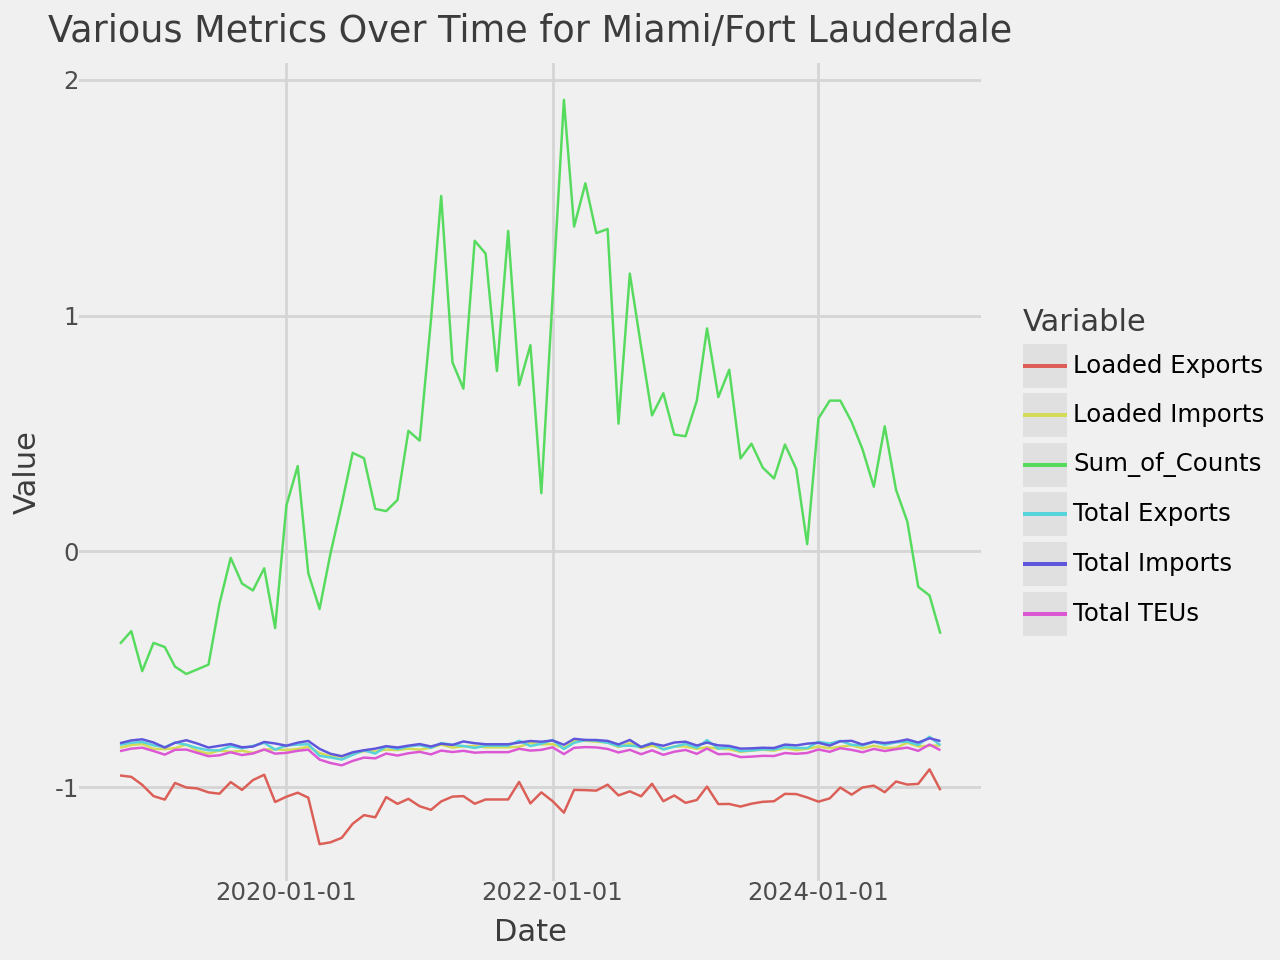
\includegraphics[width=0.8\textwidth]{timeseries_1.png}
		\end{figure}
	
		\begin{figure}[H]
			\caption{\label{timeseries_2} Redadas en el puerto de Fort Lauderdale}
			\centering
			\hspace*{1cm}
			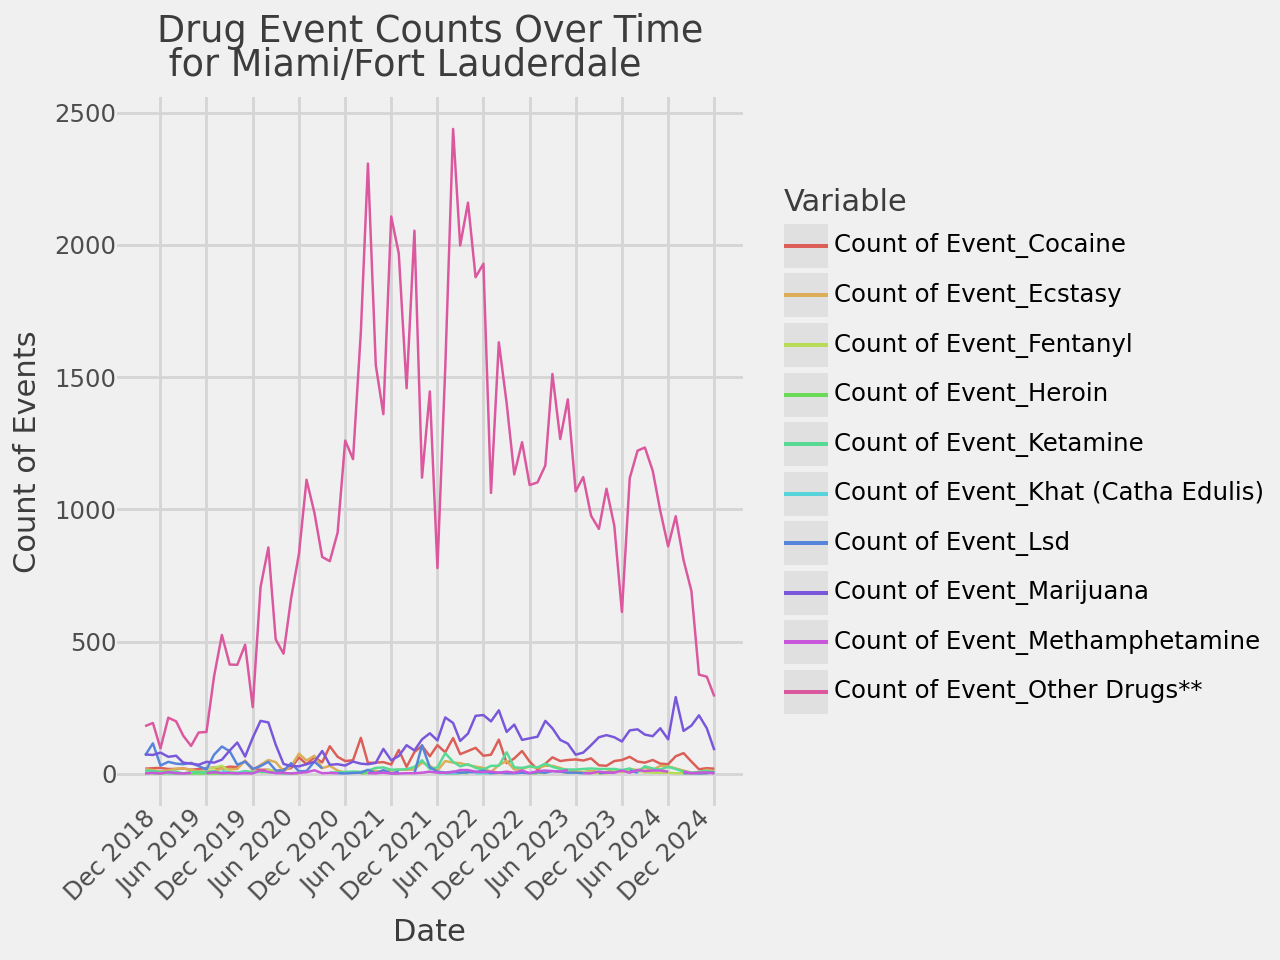
\includegraphics[width=0.8\textwidth]{timeseries_2.png}
		\end{figure}
	
		\begin{figure}[H]
			\caption{\label{timeseries_6} Redadas incautando cocaína por puerto}
			\centering
			\hspace*{1cm}
			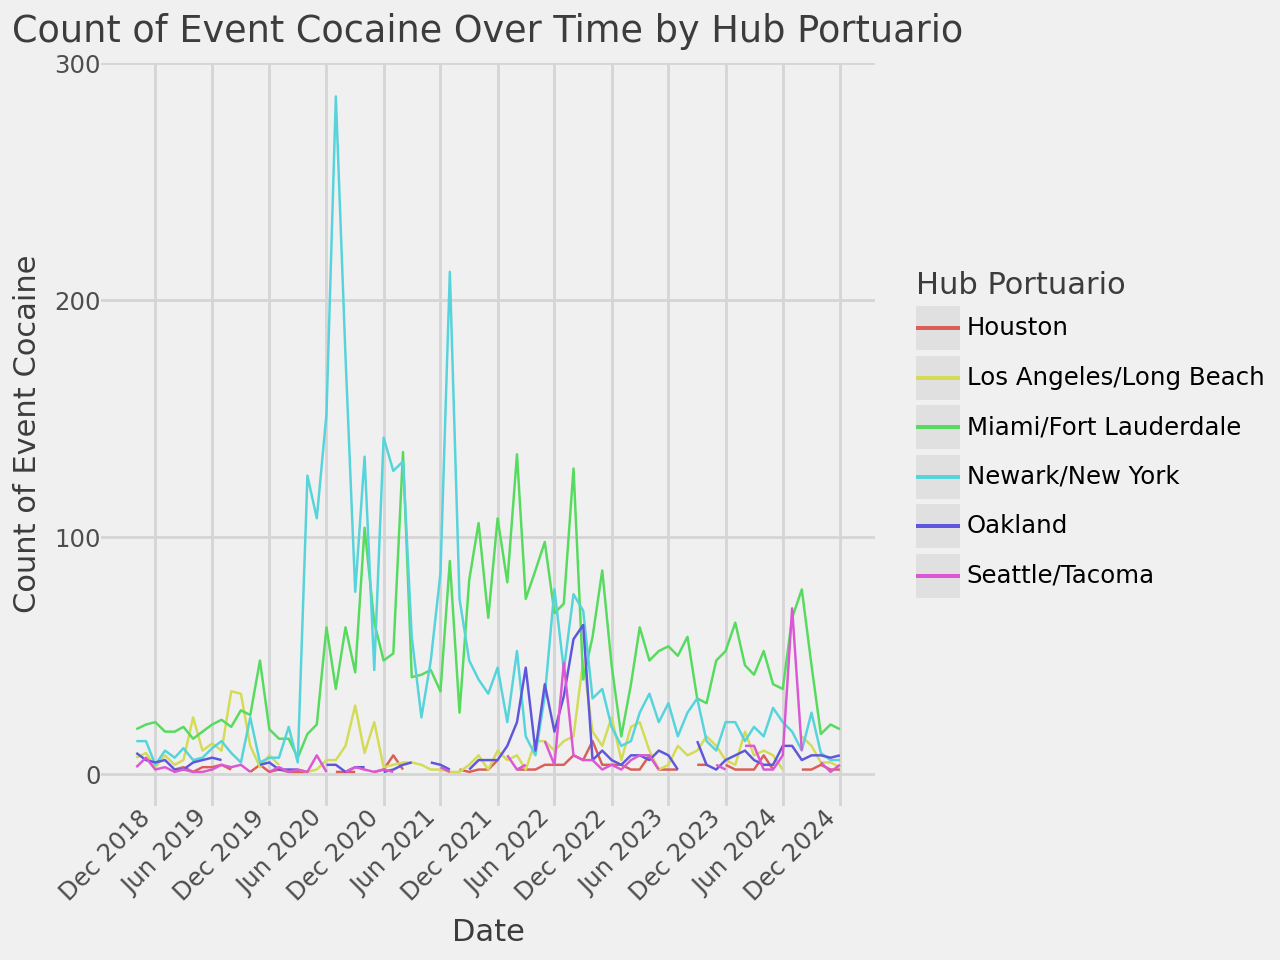
\includegraphics[width=0.8\textwidth]{timeseries_6.png}
		\end{figure}
	
		En la figura \ref{timeseries_6} se muestra la cantidad total de redadas de cocaína. Véase que los datos aportados están en valor absoluto (y se dejan las figuras \ref{timeseries_7} y  \ref{timeseries_8} para comparar visualmente la escala entre ellas).
		
		\begin{figure}[H]
			\caption{\label{timeseries_7} Redadas incautando éxtasis por puerto}
			\centering
			\hspace*{1cm}
			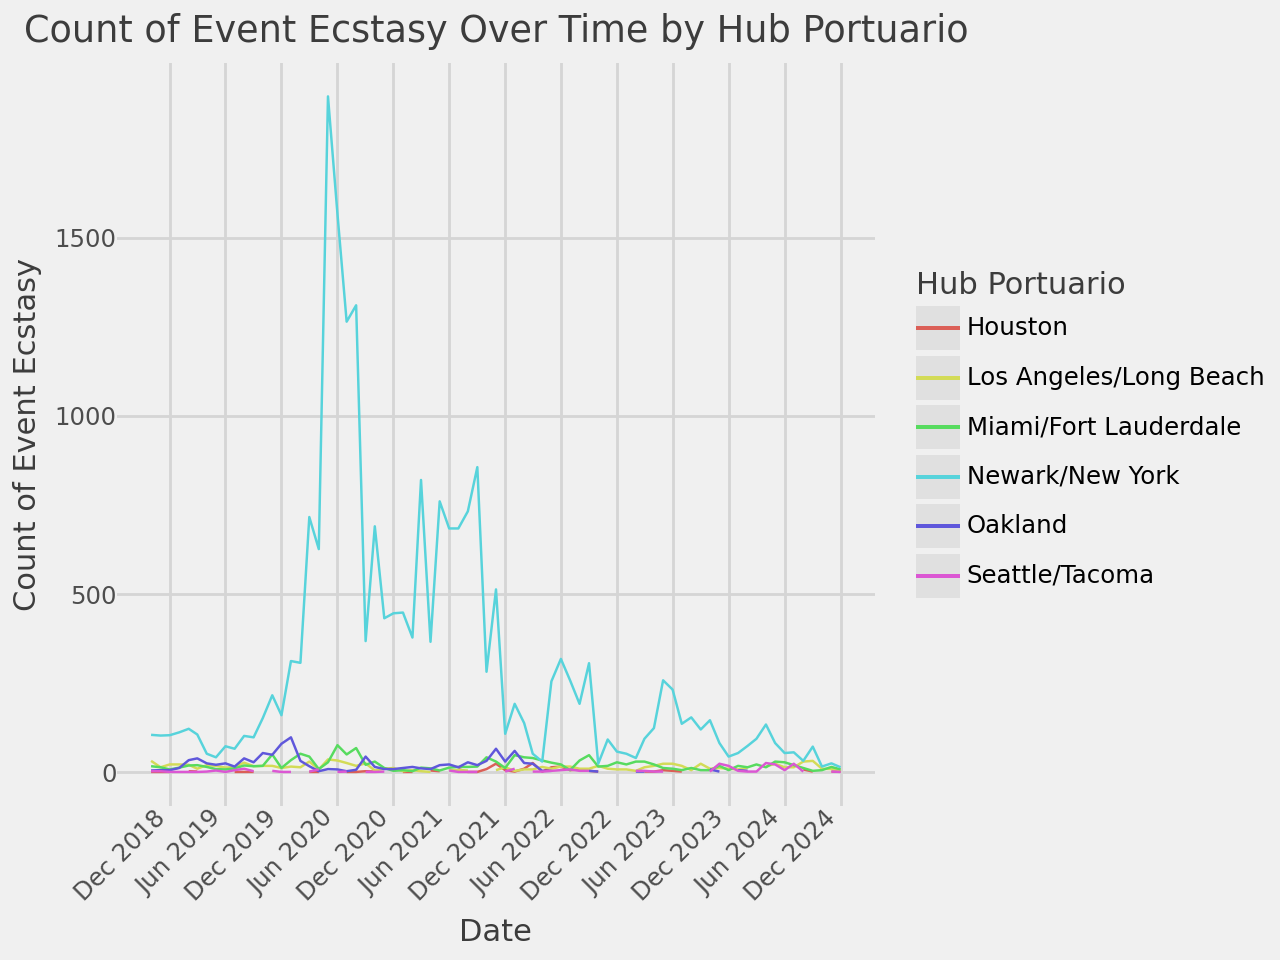
\includegraphics[width=0.8\textwidth]{timeseries_7.png}
		\end{figure}
	
		\begin{figure}[H]
			\caption{\label{timeseries_8} Redadas incautando heroína por puerto}
			\centering
			\hspace*{1cm}
			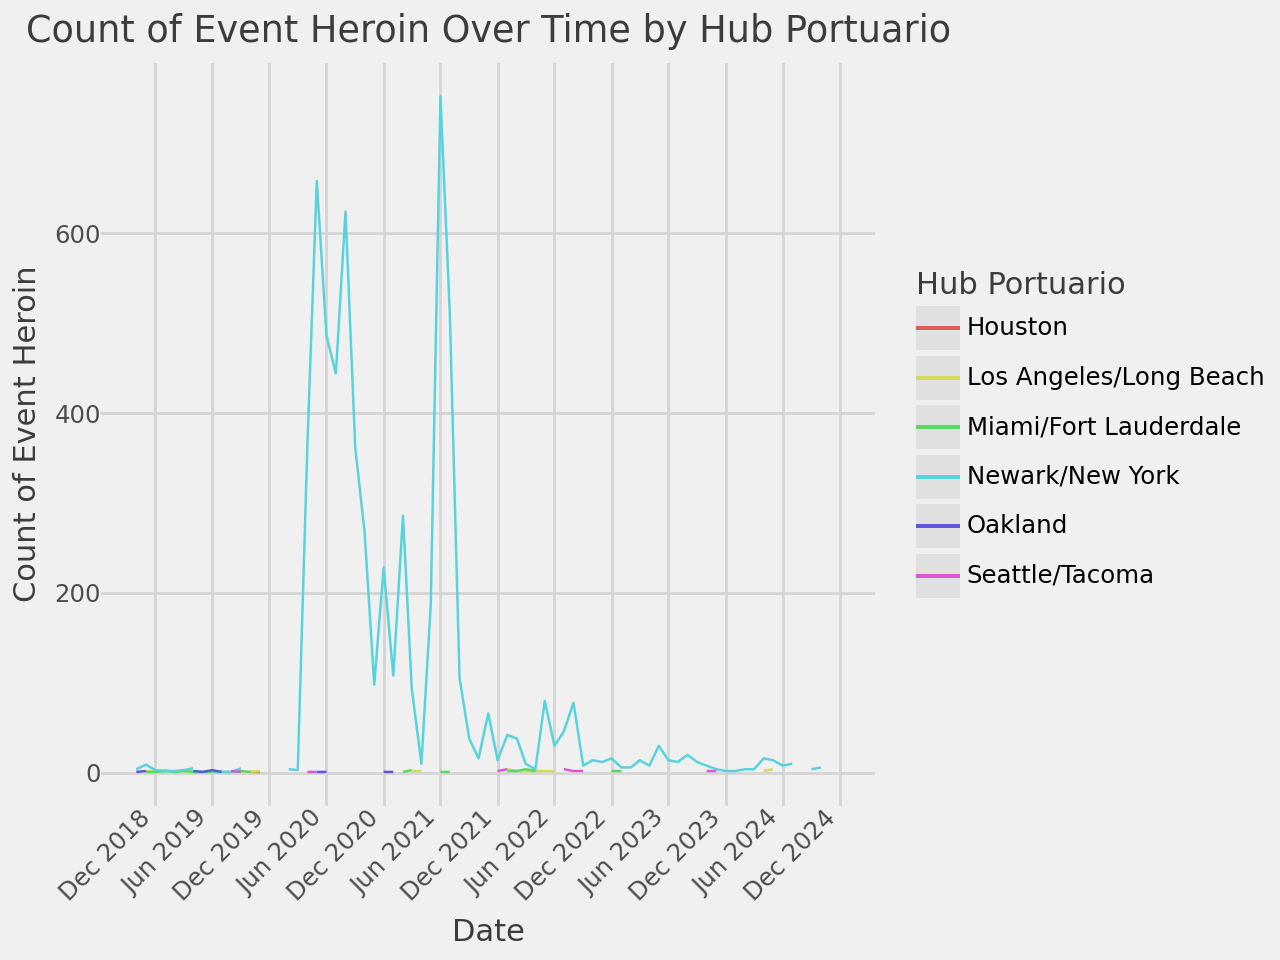
\includegraphics[width=0.8\textwidth]{timeseries_8.png}
		\end{figure}
	
		Sin embargo, si hay una categoría que resulta ser de la que más redadas hay es la considerada como "otras drogas" de las cuales no se especifica nada al respecto en los documentos originales. Véase la figura \ref{timeseries_9} también en valores absolutos por puerto.
		
		\begin{figure}[H]
			\caption{\label{timeseries_9} Redadas incautando otras drogas por puerto}
			\centering
			\hspace*{1cm}
			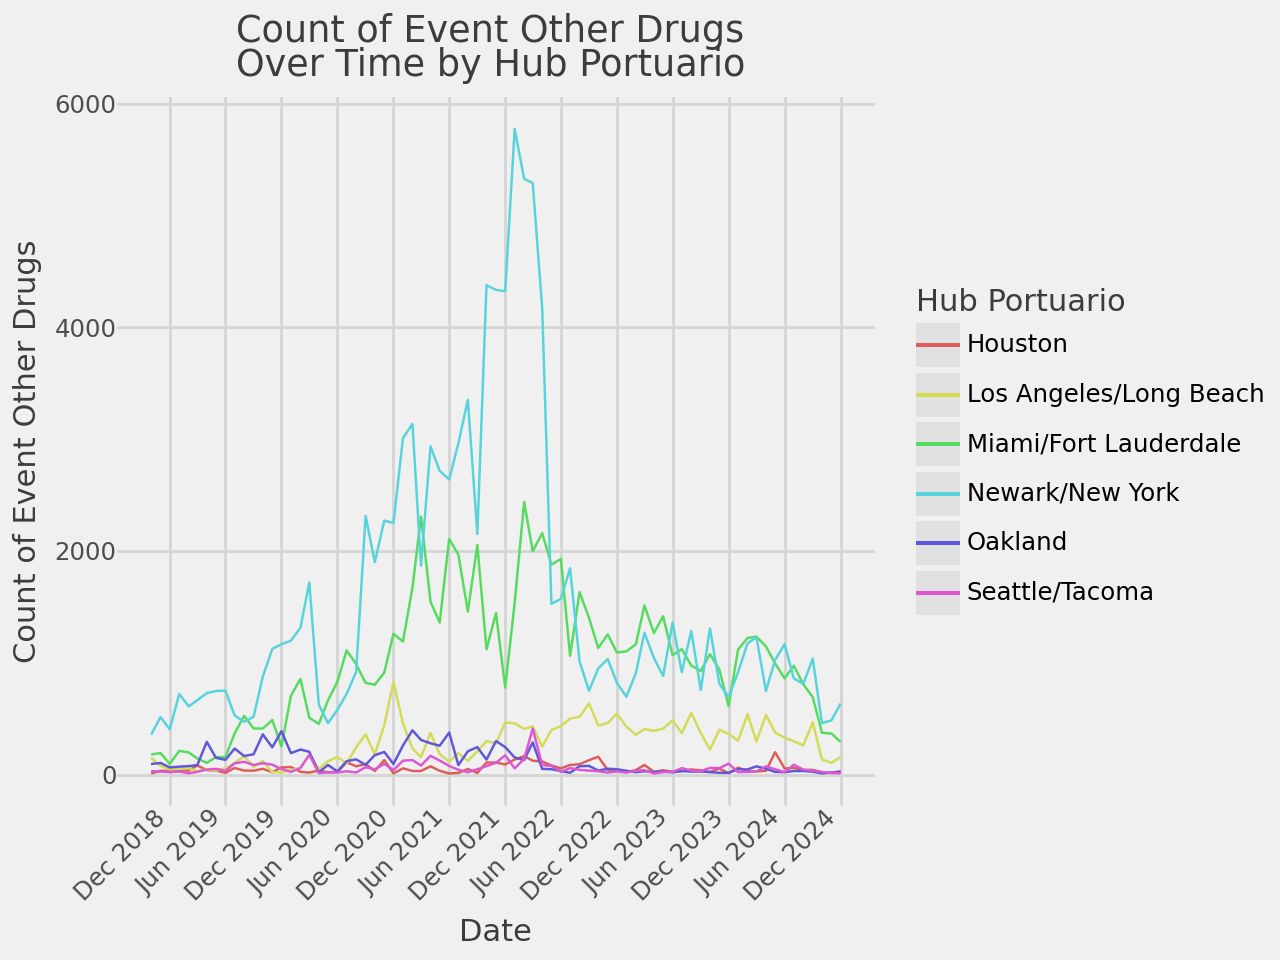
\includegraphics[width=0.8\textwidth]{timeseries_9.png}
		\end{figure}
	
		\underline{Análisis de Port Everglades}\\
		Port Everglades es como se conoce al puerto de Fort Lauderdale (en el hub portuario de Miami).
		
		Tras unas pequeñas demostraciones del comportamiento en función del tiempo de los distintos puertos, se tuvo en consideración la representación visual para variables respecto a este último puerto (véanse las figuras \ref{hist_1} y \ref{hist_2}).
		
		\begin{figure}[H]
			\caption{\label{hist_1} Distribución por número de redadas por cada mes en Fort Lauderdale}
			\centering
			\hspace*{1cm}
			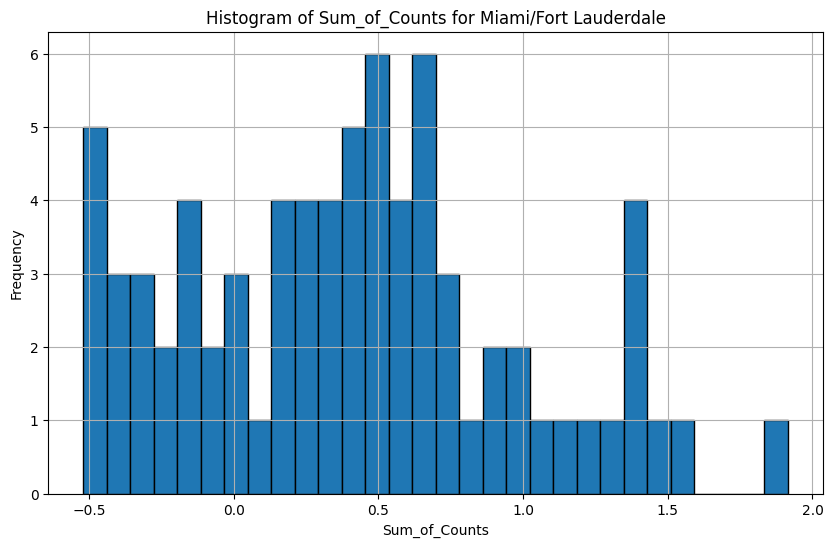
\includegraphics[width=0.8\textwidth]{hist_1.png}
		\end{figure}
	
		\begin{figure}[H]
			\caption{\label{hist_2} Distribución por número de TEUs por cada mes en Fort Lauderdale}
			\centering
			\hspace*{1cm}
			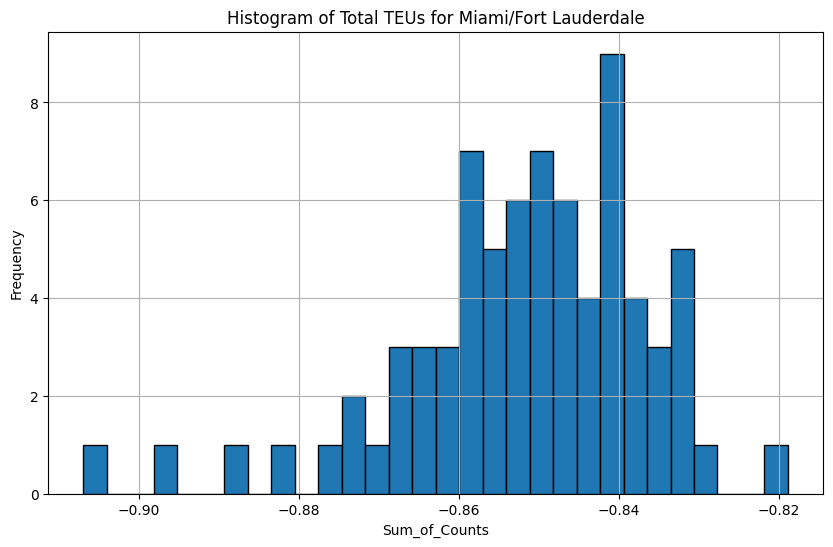
\includegraphics[width=0.8\textwidth]{hist_2.png}
		\end{figure}
	
		Por último, quiero destacar el perfecto comportamiento bimodal que se obtuvo del total de redadas del Gran Los Ángeles (figura  \ref{hist_3})
		
		\begin{figure}[H]
			\caption{\label{hist_3} Distribución por número de redadas por cada mes en Los Ángeles}
			\centering
			\hspace*{1cm}
			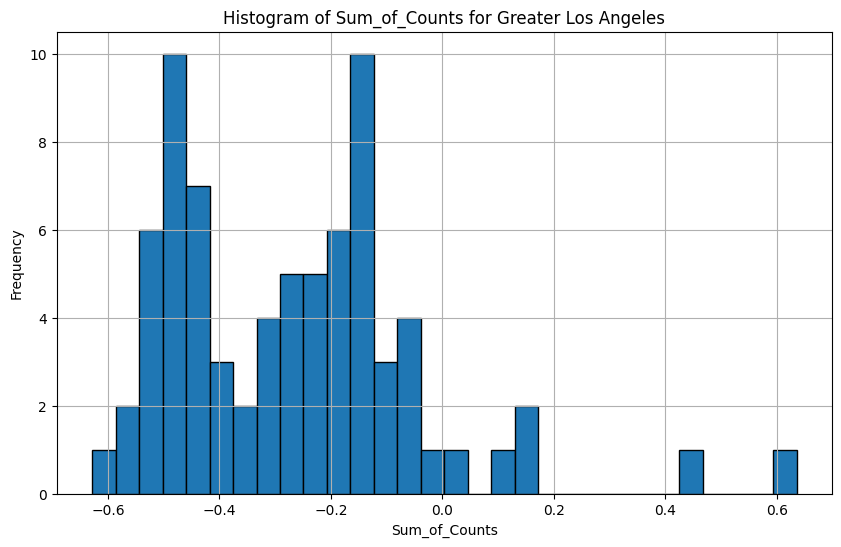
\includegraphics[width=0.8\textwidth]{hist_3.png}
		\end{figure}
	
		Es un caso a destacar por la forma de la distribución y, sobre todo, porque son datos obtenidos del CBP de Los Angeles (es decir, no se trata de una fusión de datos de Los Ángeles y Long Beach que pudieran dar lugar a ello).
		
		
		\underline{Matrices de correlación de datos}\\
		Teniendo en cuenta que el propósito de este trabajo es generar un modelo que pudiese anticipar la droga incautada (sea la cantidad, el número de redadas, por tipo, etc) a partir de la actividad en un puerto (contenedores movilizados), resulta evidente generar una matriz de correlaciones para observar a primera vista si existía alguna variable que fuera fácilmente representante del "target". En las figuras \ref{matriz_corr_1} y \ref{matriz_corr_2} se muestra una relación entre las posibles variables predictoras y variables objetivo para los puertos de Newark y Fort Lauderdale, respectivamente.
		
		\begin{figure}[H]
			\caption{\label{matriz_corr_1} Correlación entre variables predictoras y potenciales variables objetivo para el puerto de Newark}
			\centering
			\hspace*{1cm}
			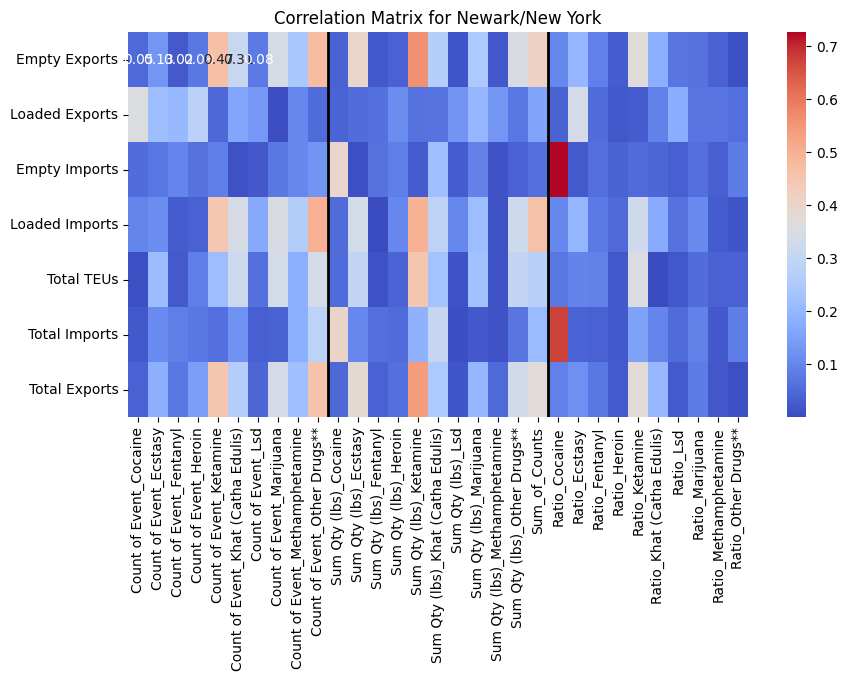
\includegraphics[width=0.8\textwidth]{matrix_corr_1.png}
		\end{figure}
	
		\begin{figure}[H]
			\caption{\label{matriz_corr_2} Para el puerto de Fort Lauderdale}
			\centering
			\hspace*{1cm}
			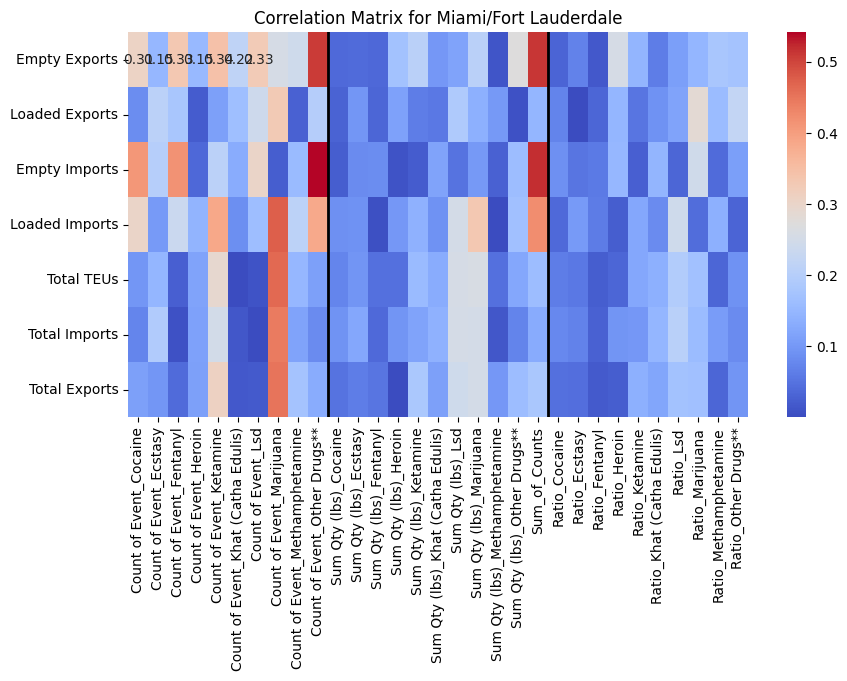
\includegraphics[width=0.8\textwidth]{matrix_corr_2.png}
		\end{figure}
		
		La figura \ref{matriz_corr_3} muestra un ejemplo de correlación entre variables predictoras para el caso del puerto de Newark (se ha comprobado que el comportamiento es igual para el resto de puertos).
		
		\begin{figure}[H]
			\caption{\label{matriz_corr_3} Correlación entre predictores para el puerto de Newark}
			\centering
			\hspace*{1cm}
			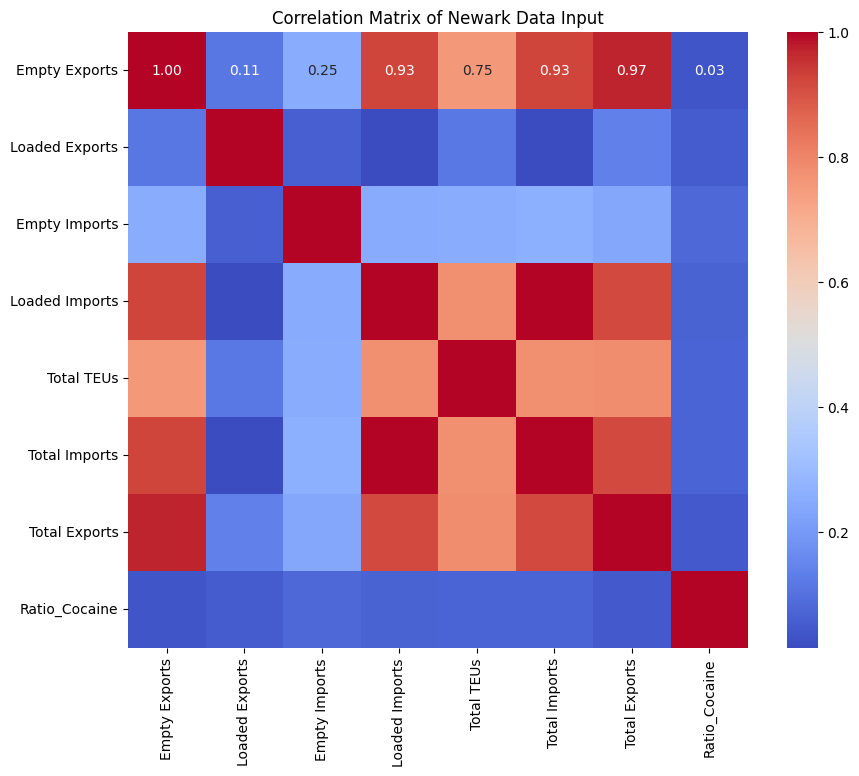
\includegraphics[width=0.8\textwidth]{matrix_corr_3.png}
		\end{figure}
	
		La lógica indica que exista una fuerte correlación entre Total Imports y Loaded Imports, no así con Total Exports, cuya correlación con éstas es incluso mayor que con Total TEUs.
		
		% Comparacion entre grupos: Graficos de barras o violin plots.
		
		Dada la poca claridad respecto a la finalidad del problema, se llegó a plantear distintos enfoques a distintos niveles. Es decir, se barajó un modelo para un puerto en concreto, para varios puertos por separado o con todos a la vez. Considerando o no sus variables geográficas, qué tipo de droga analizar. Todo ello ha sido recopilado a lo largo de esta subsección que concluye con una pequeña amalgama de mapas y otras visualizaciones.
		
		Por ejemplo, se estudió la cantidad de contenedores vacíos (y cargados) \ref{loaded_vs_imports_ports} que gestionaba cada puerto, junto con la variación temporal del total de contenedores gestionados por los mismos \ref{total_teus_ports}.
		
		\begin{figure}[H]
			\caption{\label{total_teus_ports} Serie temporal con TEUs gestionados por los puertos}
			\centering
			\hspace*{1cm}
			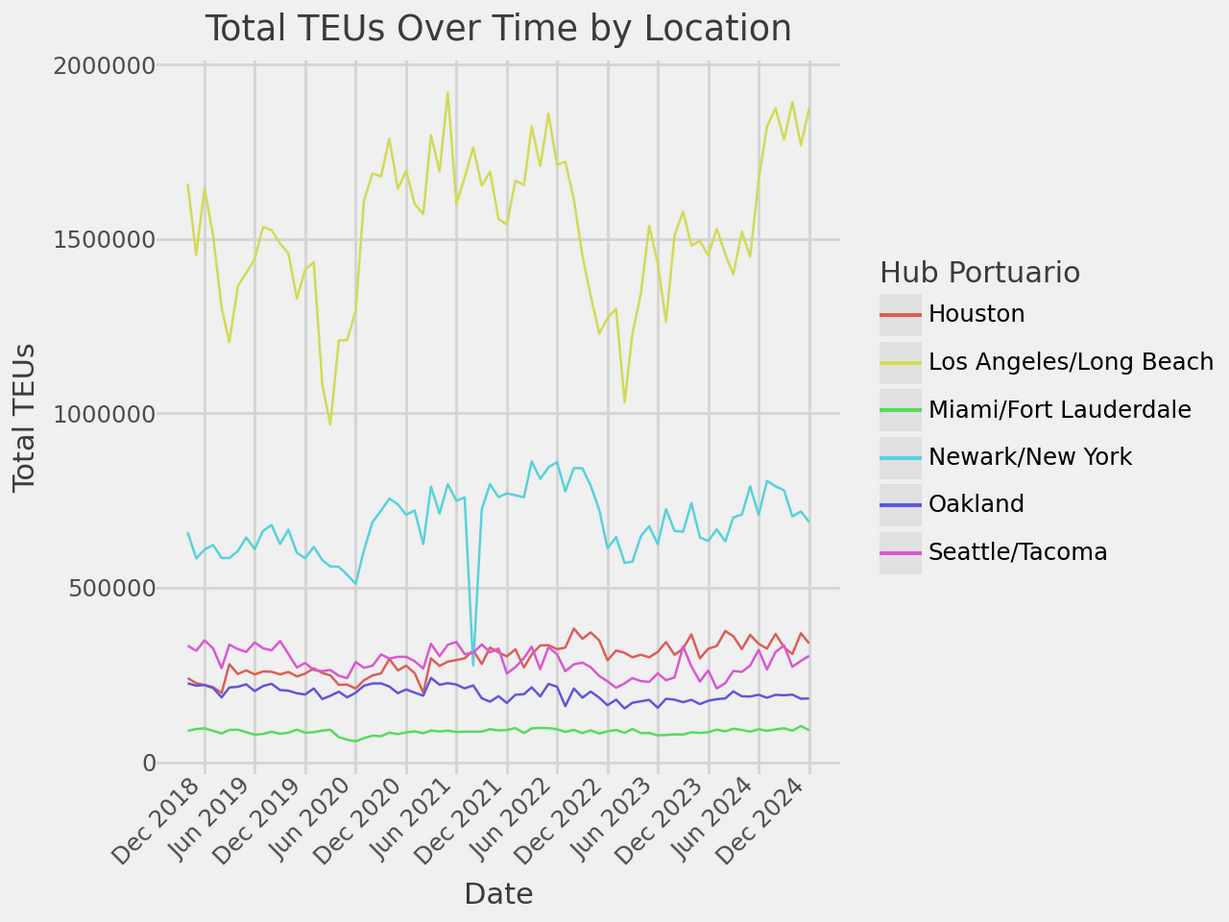
\includegraphics[width=0.8\textwidth]{total_teus_ports.png}
		\end{figure}
		
		
		\underline{Mapas geográficos}\\
		Debido a ciertos problemas a la hora de visualizar en un mapa los gráficos de tipo pie chart, se renunció a ello. La separación entre los gráficos \ref{loaded_vs_imports_ports} y \ref{map_bubble_1} viene a dar cuenta de ello.
		
		\begin{figure}[H]
			\caption{\label{loaded_vs_imports_ports} Contenedores gestionados por puertos por tipo: Vacío o Cargado}
			\centering
			\hspace*{1cm}
			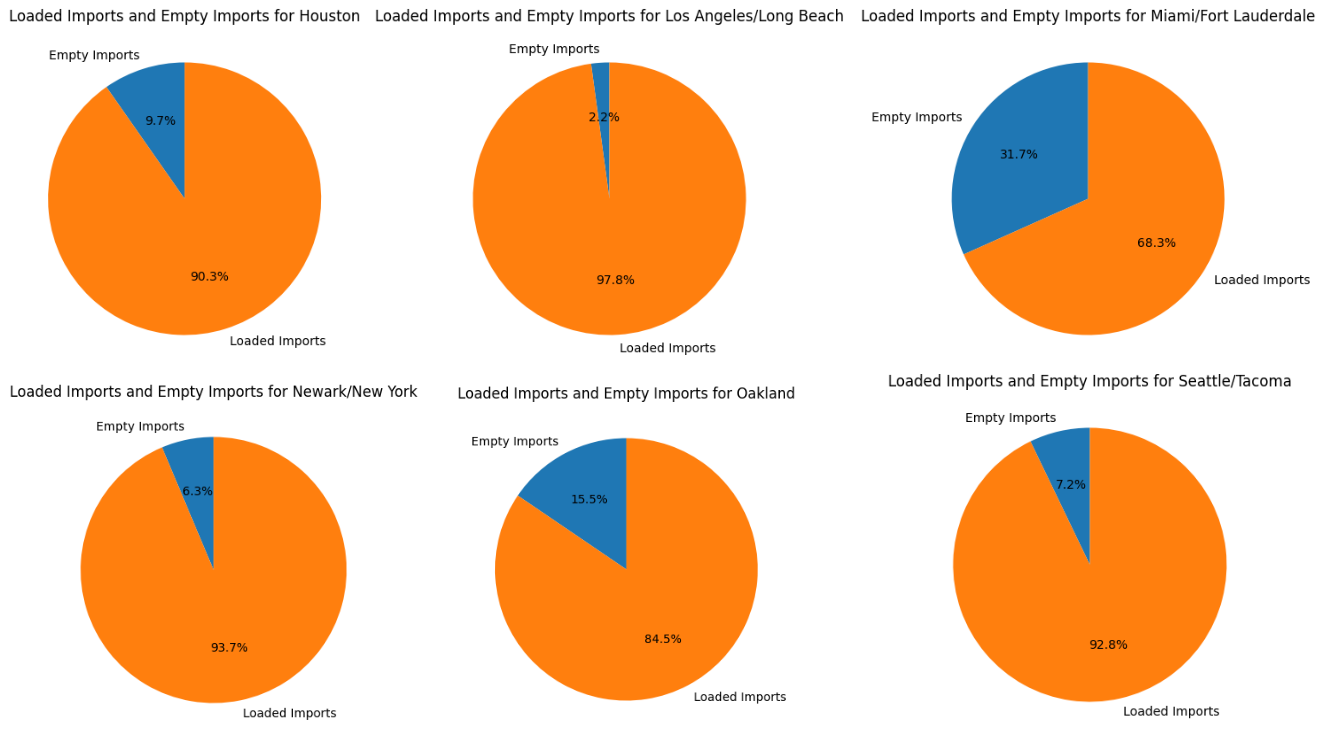
\includegraphics[width=0.8\textwidth]{loaded_vs_imports_ports.png}
		\end{figure}
	
		
		\begin{figure}[H]
			\caption{\label{map_bubble_1} }
			\centering
			\hspace*{1cm}
			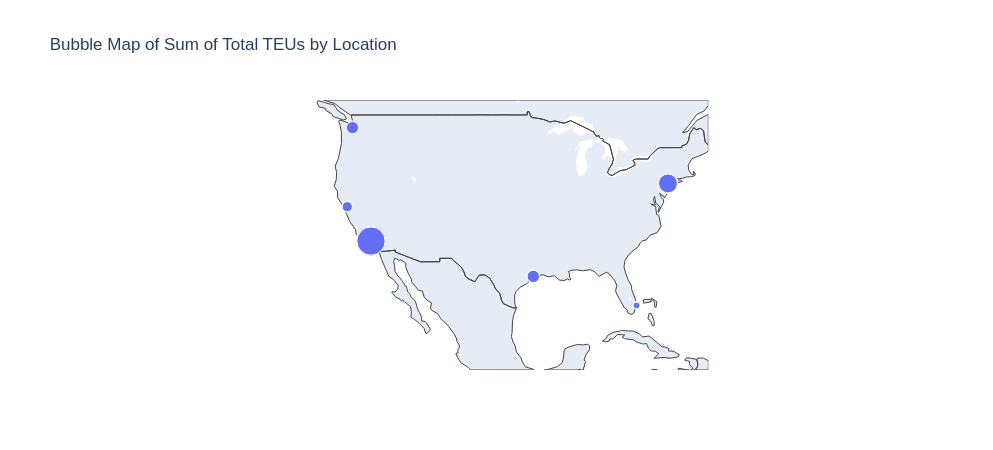
\includegraphics[width=\textwidth]{map_bubble_1.png}
		\end{figure}

		Pese a lo comentado anteriormente, si que se puede realizar un análisis de la situación de los puertos con más actividad (Los Ángeles a la cabeza), al igual que, como se irá viendo a continuación, hacerlo para cada tipo de droga y cada puerto.
		
		\begin{figure}[H]
			\caption{\label{map_bubble_2} }
			\centering
			\hspace*{1cm}
			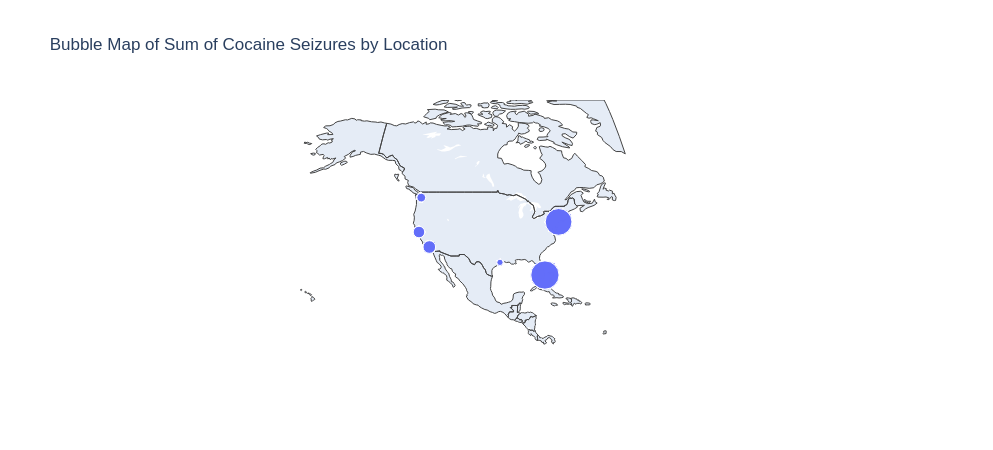
\includegraphics[width=\textwidth]{map_bubble_2.png}
		\end{figure}
	
		\begin{figure}[H]
			\caption{\label{map_bubble_3} }
			\centering
			\hspace*{1cm}
			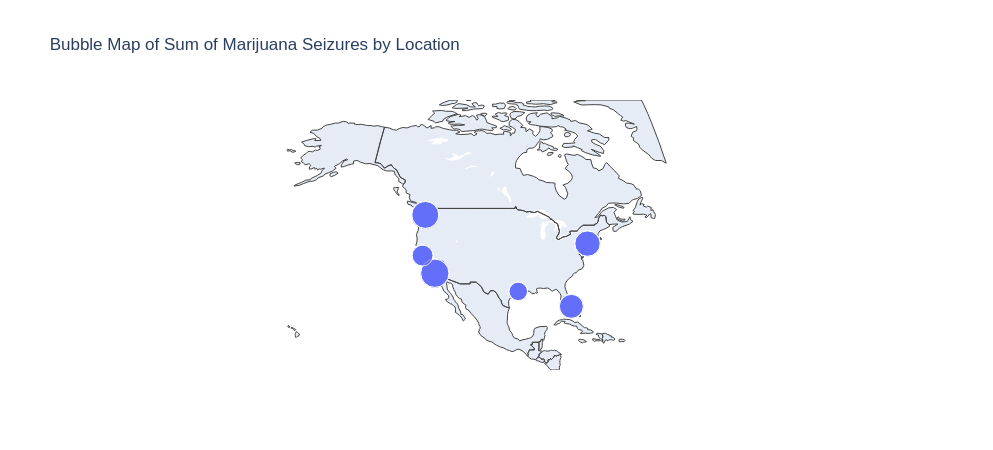
\includegraphics[width=\textwidth]{map_bubble_3.png}
		\end{figure}
	
		\begin{figure}[H]
			\caption{\label{map_bubble_4} }
			\centering
			\hspace*{1cm}
			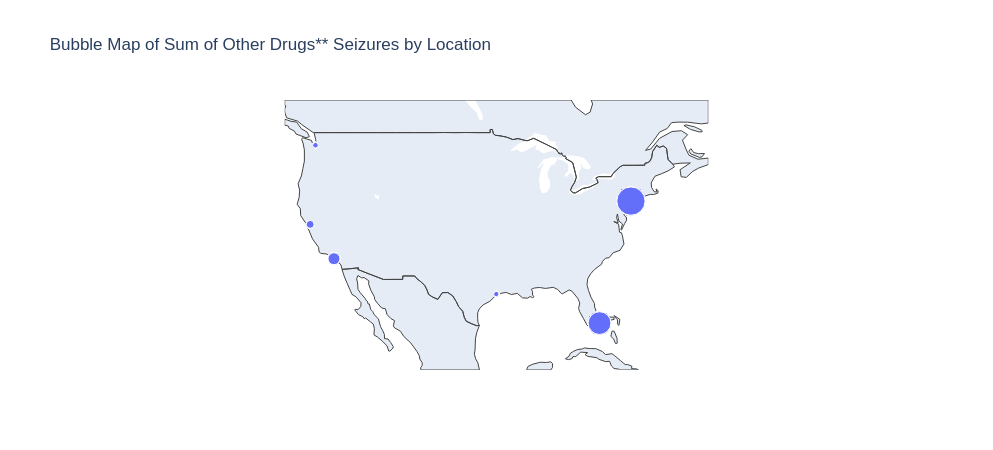
\includegraphics[width=\textwidth]{map_bubble_4.png}
		\end{figure}
	
		Por ejemplo, en las figuras \ref{map_bubble_2}, \ref{map_bubble_3} y \ref{map_bubble_4} se muestran el total de incautaciones para cocaína, marihuana* y otras drogas (no especificadas) incautadas para cada puerto.
		
		El puerto de Newark/Nueva York es un ejemplo constante de incautaciones constantes para todos los tipos de drogas. La cocaína se incauta más la costa este (especialmente por Miami) al igual que "Other Drugs". Seguramente conocer la distribución del origen geográfico de las importaciones habría aportado más información a este trabajo. Sin embargo, atendiendo a la figura \ref{timeseries_6}, anteriormente mostrada, la comparación con número de redadas era considerablemente menor que en otros casos (Véanse \ref{timeseries_7} o \ref{timeseries_8}). Especialmente para el caso de Newark.
		
		\begin{figure}[H]
			\caption{\label{map_bubble_6} }
			\centering
			\hspace*{1cm}
			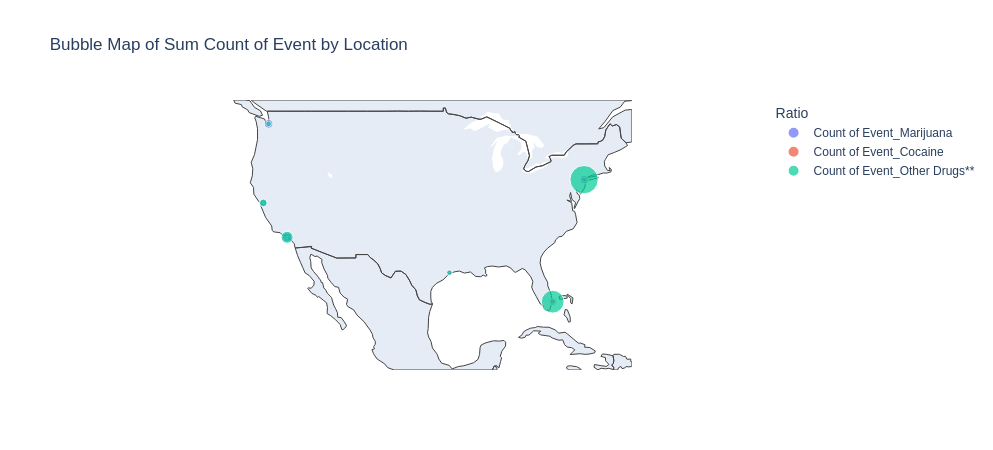
\includegraphics[width=\textwidth]{map_bubble_6.png}
		\end{figure}
		
		Por ejemplo, en la figura \ref{map_bubble_6} se muestra la cantidad de redadas por puerto para las tres principales drogas: cocaína, marihuana y otras. En todos los puertos las principales incautaciones hacen referencia a "otras", excepto para el hub portuario Seattle/Tacoma que lo hacen para marihuana. Eso sí, si observamos el radio de las burbujas del gráfico, en Seattle es muy residual.
		
		
		% Incluir pie de página para remarcar que la marihuana está legalizada en ciertos estados como California o Washington.
		
		\subsubsection{\label{preprocessing}Pre-procesamiento de los datos}
		% Limpieza, Tratamiento de Missing Values, Normalización, Estandarización, Tratamiento de Outliers...
		Este primer dataset construido, consta de 31 variables: Date (formato fecha 'YYYY-mm'), latitud y longitud (numérico float64), siete variables numéricas correspondientes a los datos portuarios, el resto de variables corresponden a los datos de incautaciones de drogas: diez variables numérica sobre "número de eventos" por droga o "Count of Events" en la versión original más una variable sumatoria de estas diez "Sum of Counts" y otras diez sobre la cantidad (en libras) incautada por droga.\
		
		\underline{Aplicaciones de scikit-learn}\\
		A la vista del primer análisis exploratorio de datos, se observaron missing values en las variables relacionadas con las incautaciones de drogas y una gran diferencia de escala entre los datos portuarios (centenas de miles de contenedores) frente a los datos de incautaciones (decenas de incautaciones). Los missing values, al tratarse de datos de fuentes de origen fiables, se imputaron a cero haciendo uso de la función SimpleImputer provista por la librería de scikit-learn. Se consideró que, aquel mes para aquella autoridad aduanera, no hubo incautación. Para seguir por esa línea, se observó una constancia en la ausencia de datos en los pares número de incautaciones-cantidad incautada. Es decir, se comprobó que si no había datos de incautación, no había datos de cantidad incautada y, por tanto, se imputase a cero. Por su parte, para la normalización de datos se aplicó la función StandardScaler también proporcionada por scikit-learn. Es a partir de aquí, que los datos con los que se van a trabajar están estandarizados a media cero y varianza uno.\
		
		\underline{Detalles del pipeline de scikit-learn}\\
		Dado que los rangos para variables de distinto tipo (incautaciones vs contenedores) eran muy diferentes entre sí, se procedió a la estandarización de los mismos mediante la implementación de pipelines en scikit-learn. Los datos numéricos ausentes se imputaron a cero (como se explicó en el párrafo anterior) y se estandarizó a una normal(0,1). Por su parte, las variables categóricas se dispusieron a ser tratadas mediante 'OneHotEncoder'*.
		
		% Incluir fragmento de código del Pipeline scikit-learn
		
		\underline{Error original en los datos de Los Angeles}\\
		En el caso de los datos obtenidos del puerto de Los Ángeles, se descubrió un error de formato en los datos de origen. En efecto, para el dato del mes de noviembre del 2020 (año fiscal 2021) se descubrió un error de formato de cambio de separador de miles (coma vs punto) en la columna 'Total TEUs'. Dado que se verificó que esta columna era igual a la suma de los valores de las columnas 'Total Imports' and 'Total Exports', se aplicó la suma de esos valores para la observación del mes de noviembre de 2020.
		
		\underline{Datos en miles para el puerto de Newark}\\
		Por su parte, resultó que los datos obtenidos para el puerto de Newark (Área Metropolitana de Nueva York-Nueva Jersey) estaban contados en miles (de contenedores). Para resolverlo, se multiplicaron estos valores por mil aparte del resto de datos para después, ser reintegrados \cite[]{}. Posiblemente el problema de integración se tratase de una incompatibilidad entre el formato europeo y americano de separador de miles.
		
		\underline{Missing Values en los datos de Fort Lauderdale}\\
		Por su parte, como se mencionó en la sección \ref{data origin}, en el caso de Fort Lauderdale, debido a las características particulares de su adquisición e integración de datos, se observaron la falta de los mismos correspondientes al último trimestre del año fiscal 2021.
		
		% Captura de pantalla para 2021 FY.
		
		Una ventaja que se tenía a la hora de poder imputar estos datos, era la posesión de todos los datos de años fiscales a nivel anual, es decir, el valor integrado de los datos mensuales \cite{Preliminary_Waterborne_Commerce_Chart_2024}. Conociendo estos datos y dado que no solo ofrecían el total de contenedores o de importaciones/exportaciones sino también qué contenedores están cargados y cuáles están vacíos, se pudo plantear el problema de la imputación de los missing values como valores MNAR, es decir, imputarlos a partir del contexto. Se aseguró que realmente los datos anuales coincidían con los datos mensuales y, en consecuencia, se fueron imputando según variables: de Loaded Imports, a Empty Exports, así hasta el total de importaciones y de exportaciones y, en último lugar, el total de TEUs (suma de las dos variables previas). En último lugar, respecto a esta operación, se imputó el mismo valor para cada mes ausente (una alternativa que se planteó fue la imputación aleatoria con una media próxima al valor imputado pero una cierta varianza incluida).
		
		% Captura de pantalla para Anual FY.
		
		\underline{Tratamiento de Outliers}\\
		Para el tratamiento de Outliers, en un primer momento se fueron estudiando caso a caso, la situación de cada uno, su contexto, etc. Intentando comprender qué valor aportaba al modelo, si pudiera ser un dato que alterase en exceso al resto o si fueran datos que simplemente estuviesen un poco más allá de las fronteras teóricas (rango intercuartil, QQ-Plot, método de las tres sigmas) fuera de lugar. Dado que el número de observaciones no era demasiado grande, en muchos casos, se limitó a que el umbral para excluir datos fuera el valor absoluto cinco de los datos normalizados. Es decir, se intentó minimizar el número de datos excluidos, pero se decidió que en algunos casos, eran necesarios para avanzar en el estudio del problema.\
		
		En la siguiente sección \ref{feature engineering} se hace referencia y se detalla la generación de nuevas variables. Entre ellas destaca el conjunto de variables de tipo "Ratio". Pese a no haberse hecho mención de ella, salvo si acaso, de pasada, será útil para detectar ciertas anomalías en los comportamientos. Esto puede servir para ver como orientar el modelo, más allá de que se acabe usando o no en éste. Aportará información de gran relevancia de forma visual. Aquí dejo una serie de gráficas estandarizadas sobre esa variable que sirve para detectar ciertos valores extremos (outliers) que serán excluidos.
		
		
		% Visualización (o datos) de media por hub portuario de incautaciones y de tráfico de contenedores.
		
		El criterio de exclusión de outliers ha sido muy laxo. Se han considerado todos aquellos valores normalizados más allá de cinco (quedando en extremos residuales de las colas de la normal) debido a la escasez de datos, intentando minimizar el número de datos a excluir.
		
		% [Tras eliminar outliers] Graficos de dispersion (scatter plots). Correlacion entre variables.
		\begin{figure}[H]
			\caption{\label{boxplot_1} Boxplot para hallar outliers en redadas de cocaína}
			\centering
			\hspace*{1cm}
			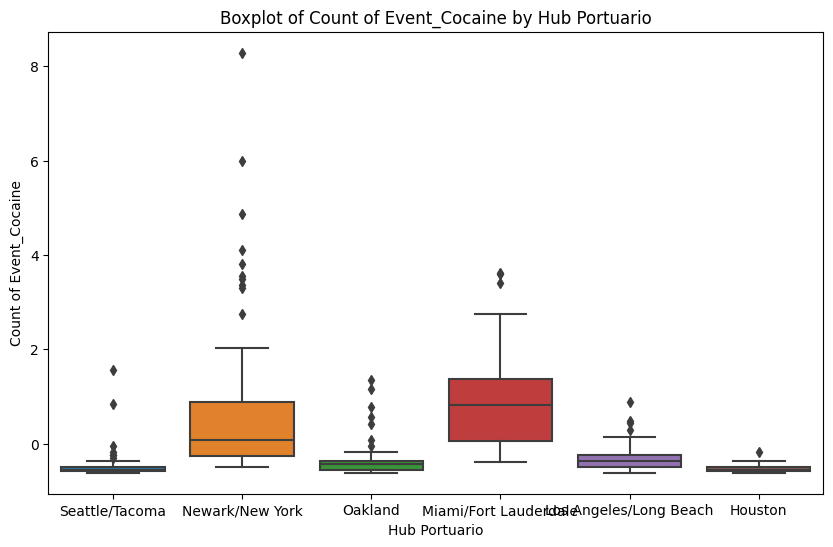
\includegraphics[width=\textwidth]{boxplot_1.png}
		\end{figure}
	
		\begin{figure}[H]
			\caption{\label{boxplot_3} Boxplot para hallar outliers en ratios de cocaína}
			\centering
			\hspace*{1cm}
			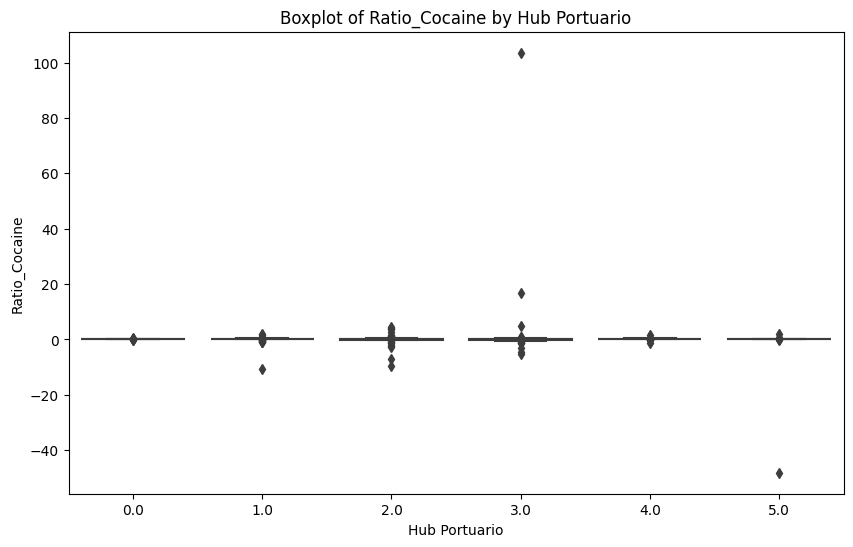
\includegraphics[width=\textwidth]{boxplot_3.png}
		\end{figure}
	
		\begin{figure}[H]
			\caption{\label{boxplot_4} Boxplot para hallar outliers en redadas de otras drogas}
			\centering
			\hspace*{1cm}
			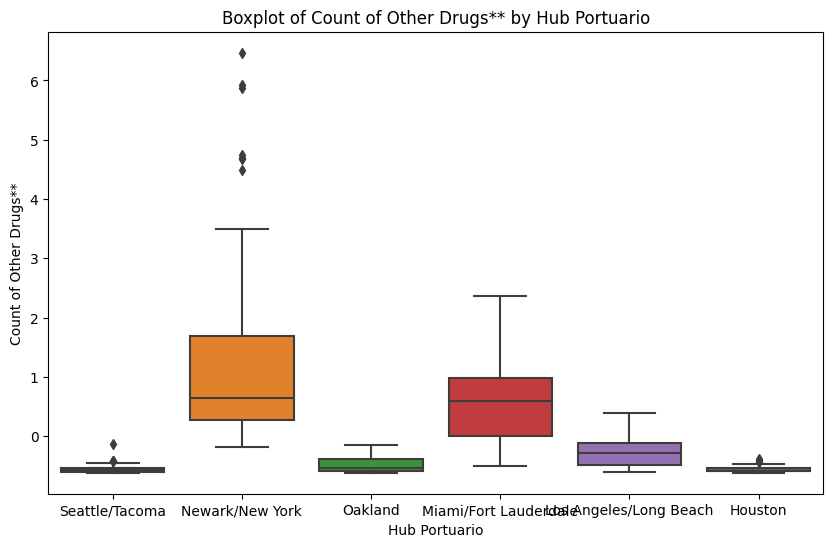
\includegraphics[width=\textwidth]{boxplot_4.png}
		\end{figure}
	
		\begin{figure}[H]
			\caption{\label{boxplot_2} Boxplot para hallar outliers en ratios de otras drogas}
			\centering
			\hspace*{1cm}
			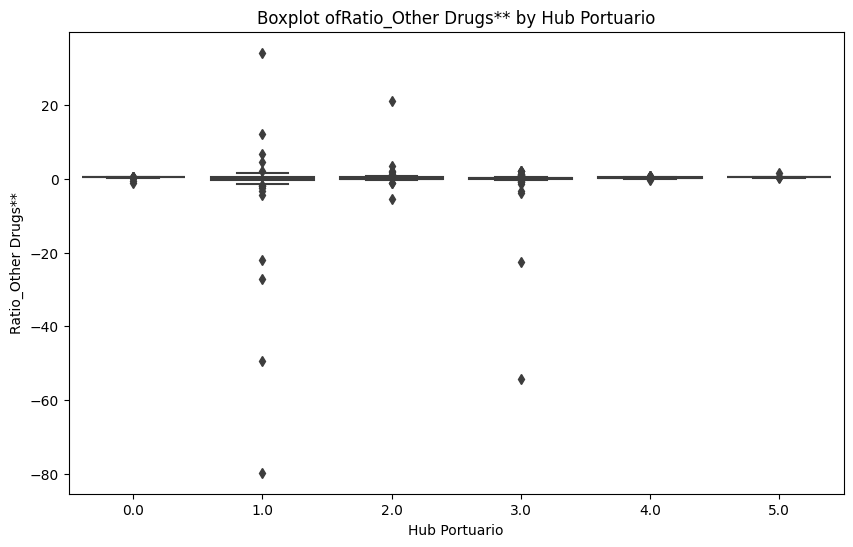
\includegraphics[width=\textwidth]{boxplot_2.png}
		\end{figure}
	
		Obsérvese en qué valores se sitúan aquellos referentes a las variables "Ratio", muy alejados del resto del grupo de valores. En cambio, para las variables "Count" la distribución es más común y aquellos valores outliers no afectan tanto a la distribución.
	
		En los pares de imágenes \ref{boxplot_1} - \ref{boxplot_3}  y \ref{boxplot_4} - \ref{boxplot_2} se muestra que la aplicación de la variable ratio tenderá a poseer datos que se alejan mucho del resto. Éstos podrían considerarse como grandes redadas, grandes operaciones de incautación de una tacada. Ello hace que algunos puertos con poca actividad ilícita detectada, tenga algunos meses especiales que sobresalgan respecto a su media. A continuación se dejan algunas visualizaciones temporales para distintos puertos en los que se observan este tipo de comportamientos.
	
		Por ejemplo, obsérvese que para el caso de redadas de cocaína, se tiene constancia de una redada a principios de 2023 en Seattle con una gran cantidad de la misma incautada \ref{st_ratio_1}:
		
		\begin{figure}[H]
			\caption{\label{st_ratio_1} Serie temporal sobre redadas de cocaína para cada puerto}
			\centering
			\hspace*{1cm}
			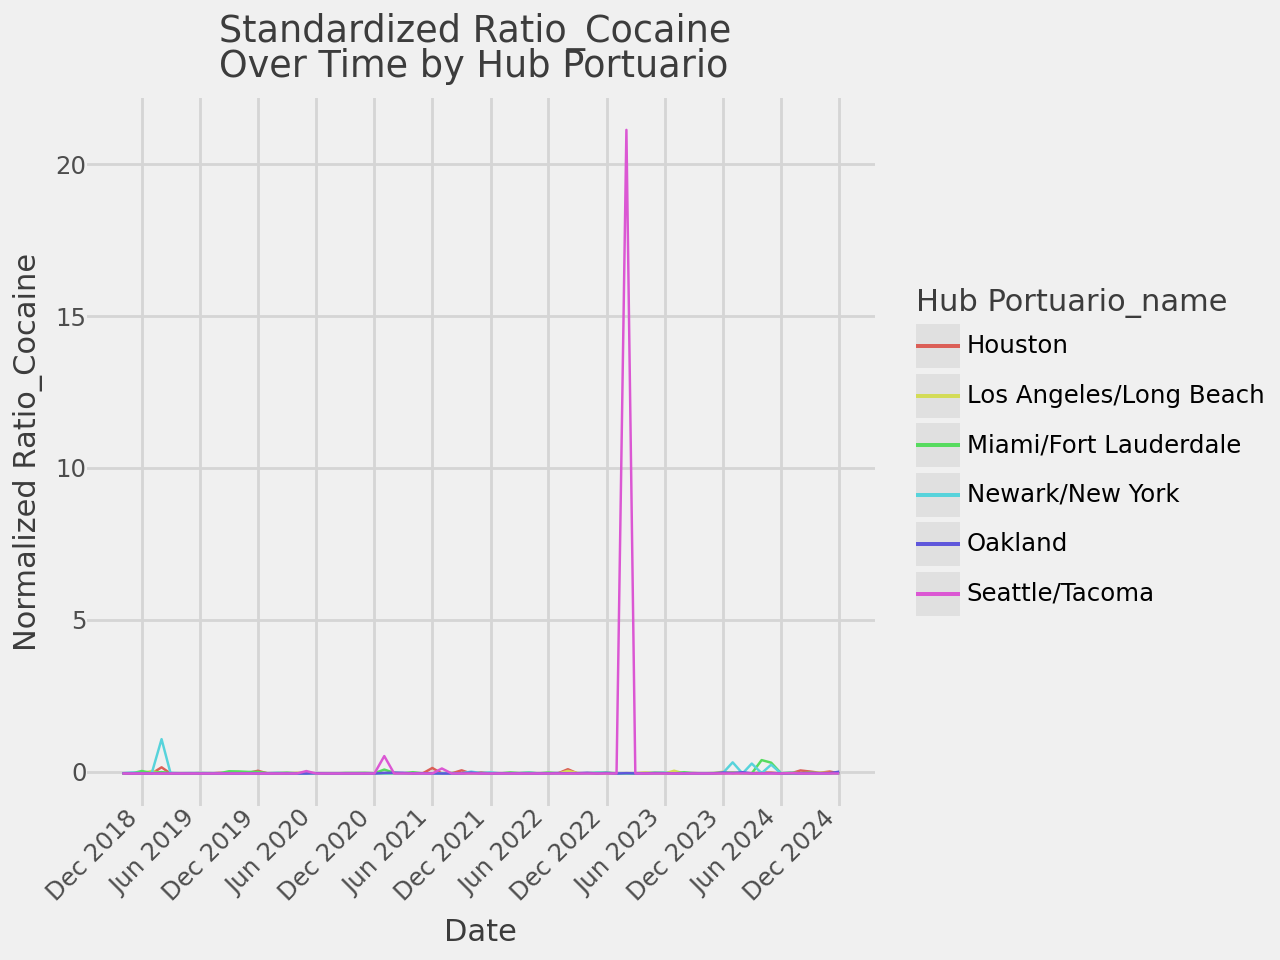
\includegraphics[width=\textwidth]{st_ratios_1.png}
		\end{figure}
	
		En el caso de redadas de marihuana \ref{st_ratio_2}, se observan grandes redadas cada cierto tiempo. Pese a tratarse de una droga de consumo legal en ciertos estados (entre ellos California o Washington), ésta se incluye en los informes del CBP sin detallar si es de contrabando o cuál es su status real.
		
		\begin{figure}[H]
			\caption{\label{st_ratio_2} Serie temporal sobre redadas de marihuana para cada puerto}
			\centering
			\hspace*{1cm}
			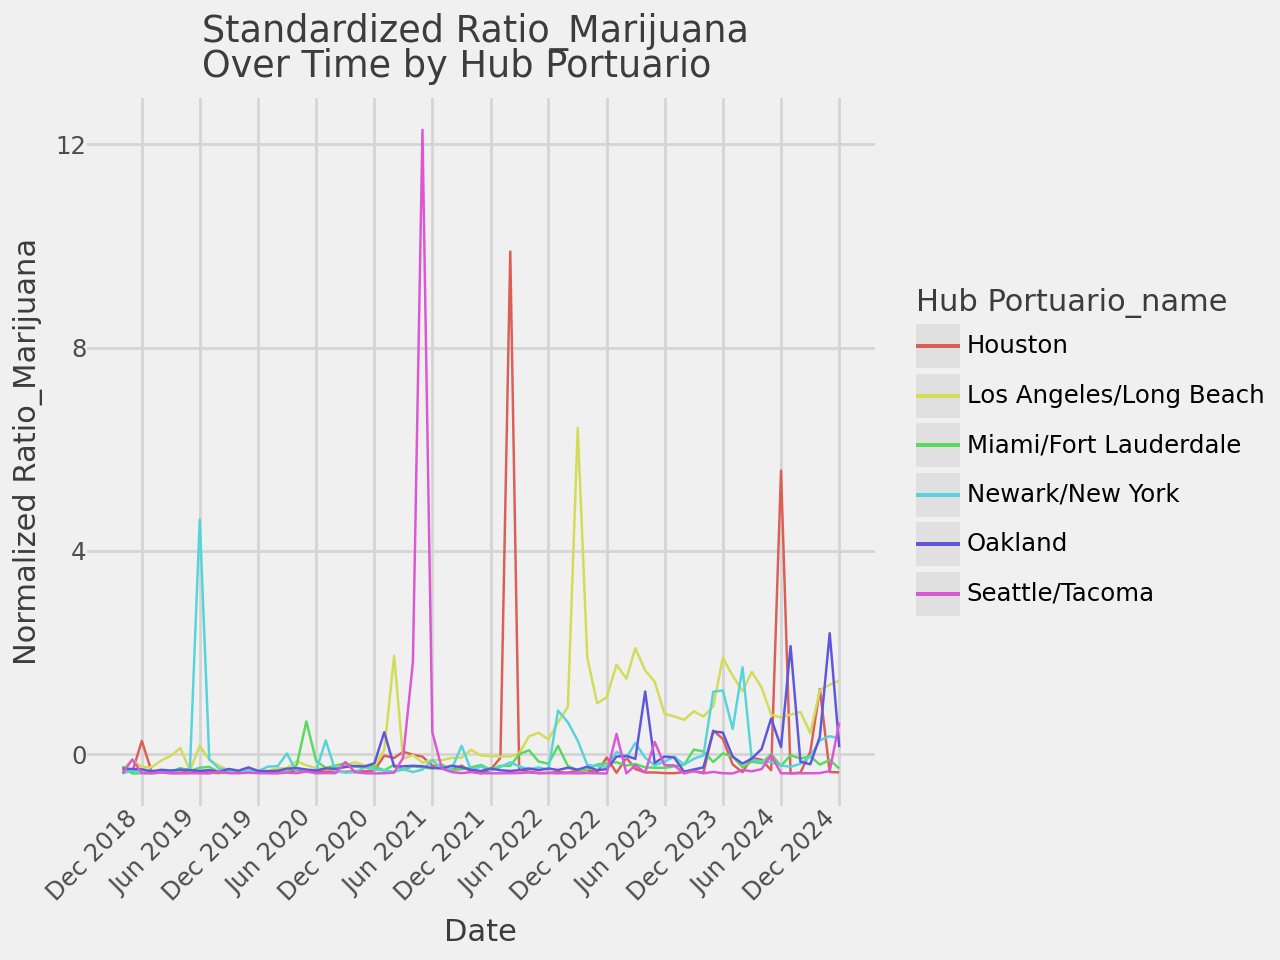
\includegraphics[width=\textwidth]{st_ratios_2.png}
		\end{figure}
	
		\underline{Ejemplo de outlier en GLA}\\
		También se muestra el comportamiento para las redadas de "Otro tipo de drogas" (Véase la figura \ref{st_ratio_3}). En este caso destaca una redada importante en el hub portuario del Gran Los Ángeles (GLA)
		
		\begin{figure}[H]
			\caption{\label{st_ratio_3} Serie temporal sobre redadas de marihuana para cada puerto}
			\centering
			\hspace*{1cm}
			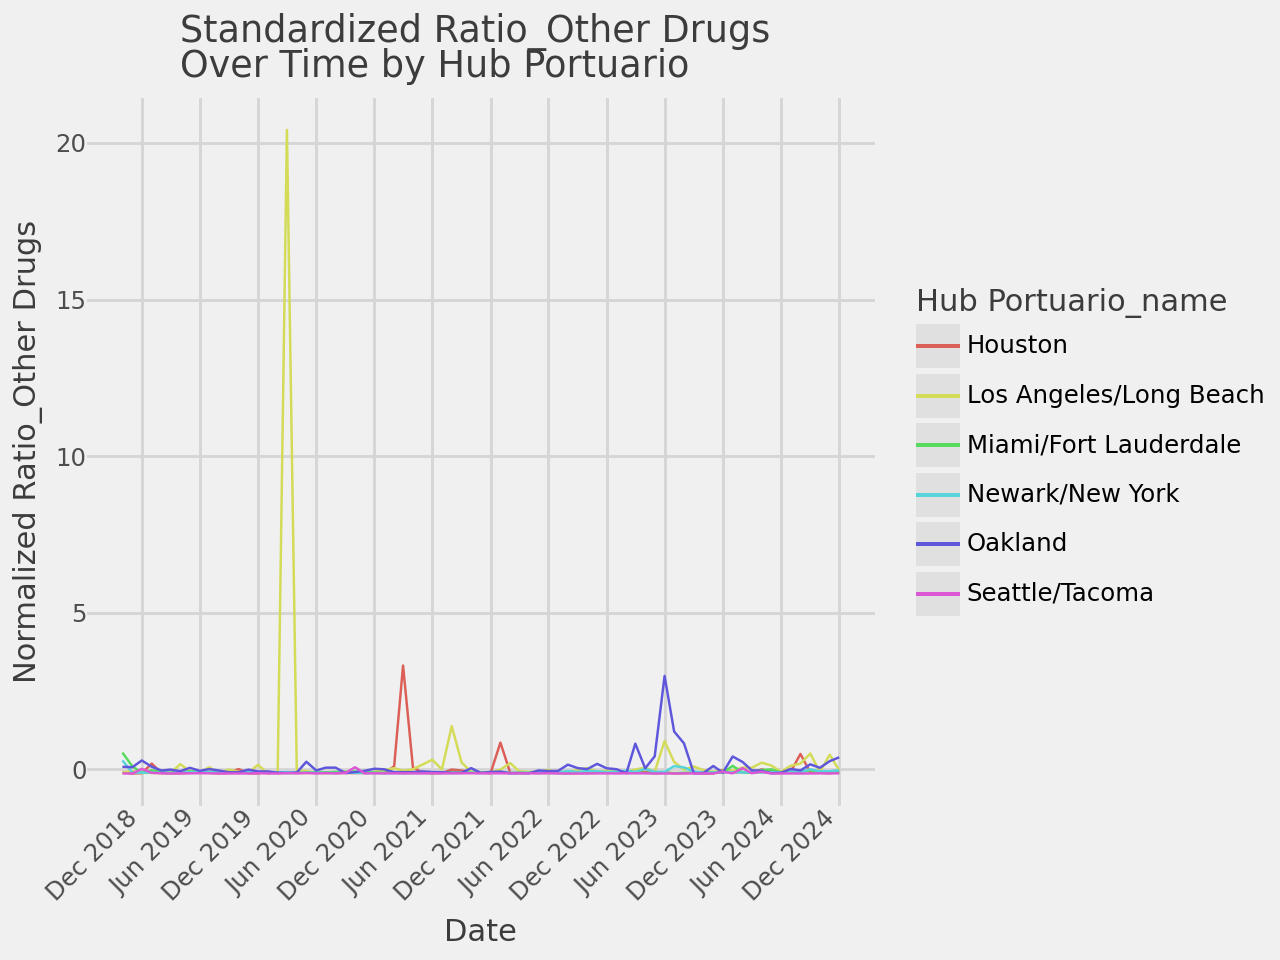
\includegraphics[width=\textwidth]{st_ratios_3.png}
		\end{figure}
	
		Este caso particular va a servir para mostrar la alteración del dataframe tras el tratamiento de la observación con este outlier.
		
	
		\subsubsection{\label{feature engineering}Ingeniería de características}
		Tras unas primeras visualizaciones y determinadas certezas respecto a los datos brutos que componían el dataset primitivo, se estimó necesario la inclusión de otras variables que fuesen generadas a partir de éstas primeras.\
		% Generación del target (y posibles alternativas)
		
		\underline{Sum of Counts}\\
		Uno de los puntos que más quebraderos de cabeza trajo respecto al desarrollo del modelo fue, por encima de todo, qué variable se usaría como target. Pese a que este punto será abordado con mayor profundidad en la sección \ref[Implementación Práctica del Modelo]{}, pronto surgió la idea de incluir una variable que agrupase todas las incautaciones (número de redadas) sin importar la categoría de la droga para un mismo mes y una misma región. Sin embargo, esto no era posible realizarlo sobre la cantidad de droga incautada (masa en libras) ya que carecía de sentido mezclar masas de distintos orígenes (se llegó a pensar en hacer la suma del valor incautado, pero también se descartó por la falta de datos al respecto y, que la influencia del mismo valor al igual que la masa generase ciertas distorsiones entre una región u otra).\ 
		
		% Sumatorio por count event de tipo de drogas:
		$$
		Sum\; of\; Counts = \sum_i C_{count\; event,i}
		$$
		%
		Donde $i$ es cada tipo de droga.
		
		\underline{Ratios por Tipo de Droga}\\
		Una vez generada la variable "Sum of Counts", era posible tener una asignación de cada puerto con la cantidad total de redadas mensuales. Pero dentro de esas redadas, en un principio, se consideró que aportaría valor el conocer cómo eran esas redadas: si lograban continuamente capturar gran cantidad de estupefacientes, si en cambio, solían ser pequeñas incautaciones con algún "premio" en forma de gran redada... Si esto dependía del tipo de droga y/o del hub portuario. Para ello se fueron creando las variables "Ratio\_" para cada tipo de droga que era el cociente entre la cantidad incautada de un tipo de droga durante un mes en una región y el número de redadas durante ese mes en esa misma región.
		
		A continuación se muestran una serie de gráficas que muestran la relación entre la cantidad de droga incautada con el número de redadas. Nótese que las figuras representadas son anteriores al análisis y exclusión de outliers:
		
		\begin{figure}[H]
			\caption{\label{graph_ratios_1} Relación entre la cantidad de cocaína incautada y el número de redadas por puerto}
			\centering
			\hspace*{1cm}
			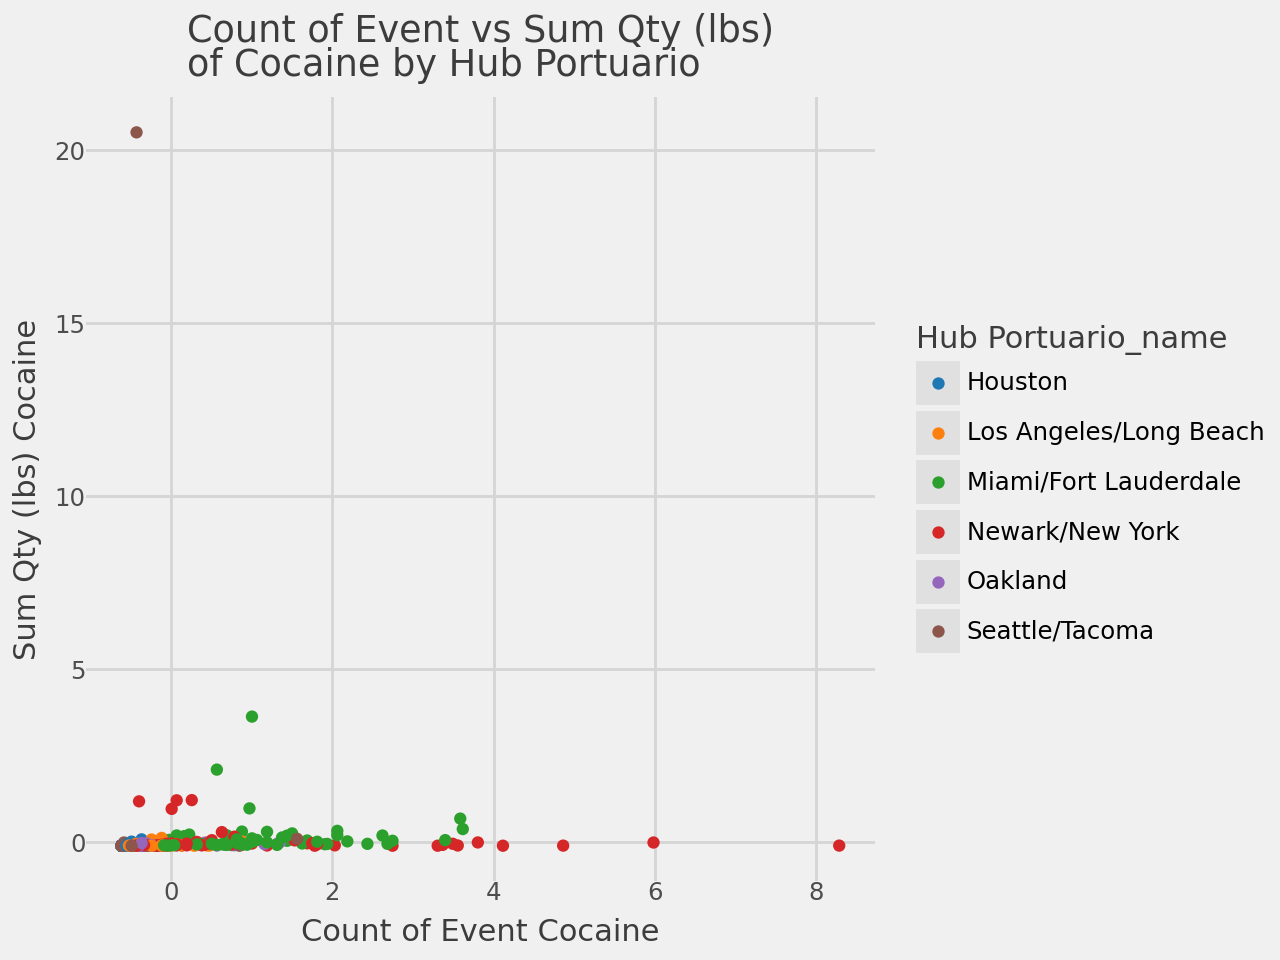
\includegraphics[width=\textwidth]{graph_ratios_1.png}
		\end{figure}
	
		\begin{figure}[H]
			\caption{\label{graph_ratios_2} Relación entre la cantidad de heroína incautada y el número de redadas por puerto}
			\centering
			\hspace*{1cm}
			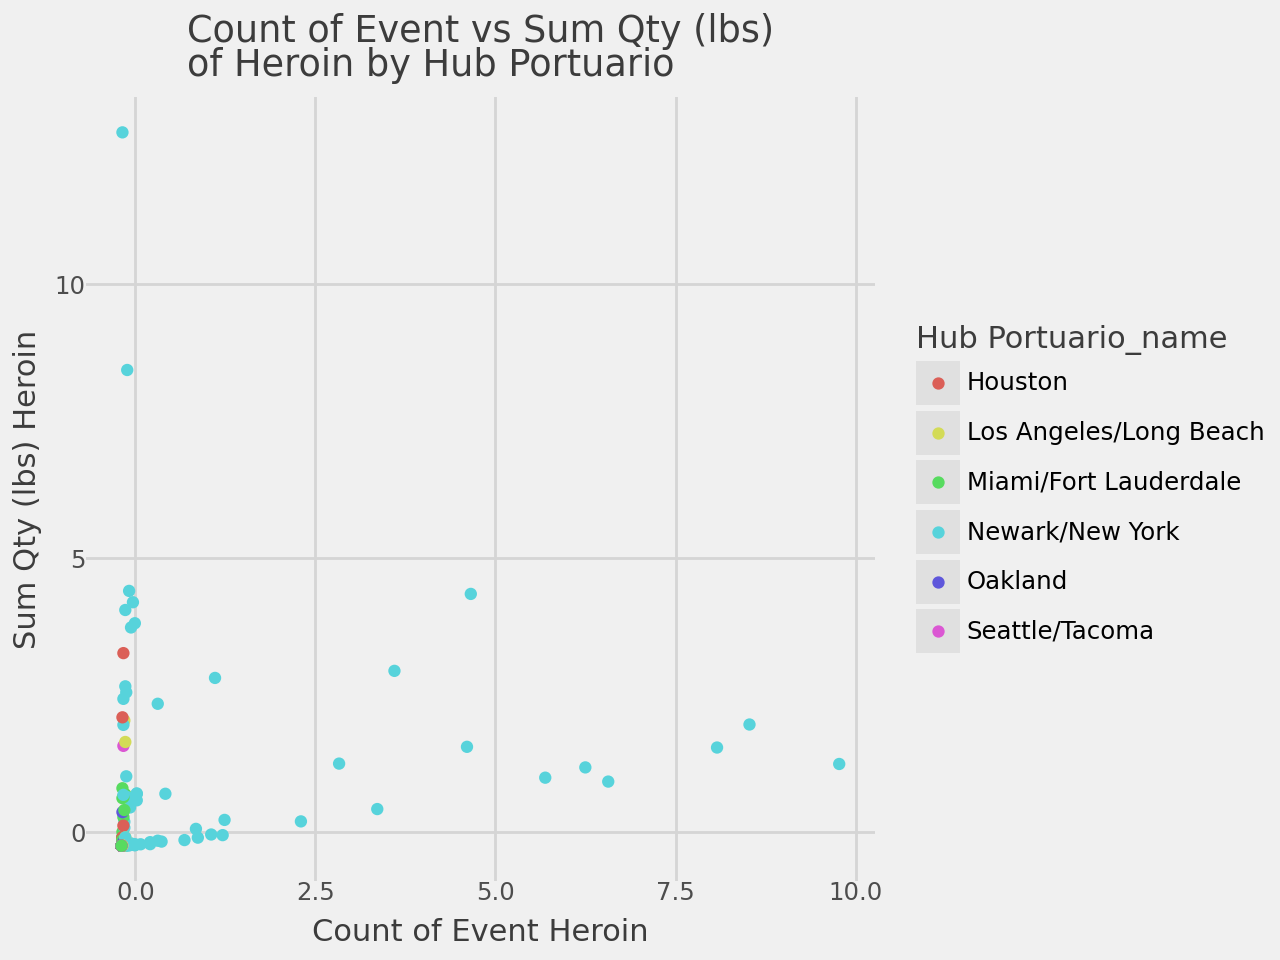
\includegraphics[width=\textwidth]{graph_ratios_2.png}
		\end{figure}
	
		\begin{figure}[H]
			\caption{\label{graph_ratios_3} Relación entre la cantidad de marihuana incautada y el número de redadas por puerto}
			\centering
			\hspace*{1cm}
			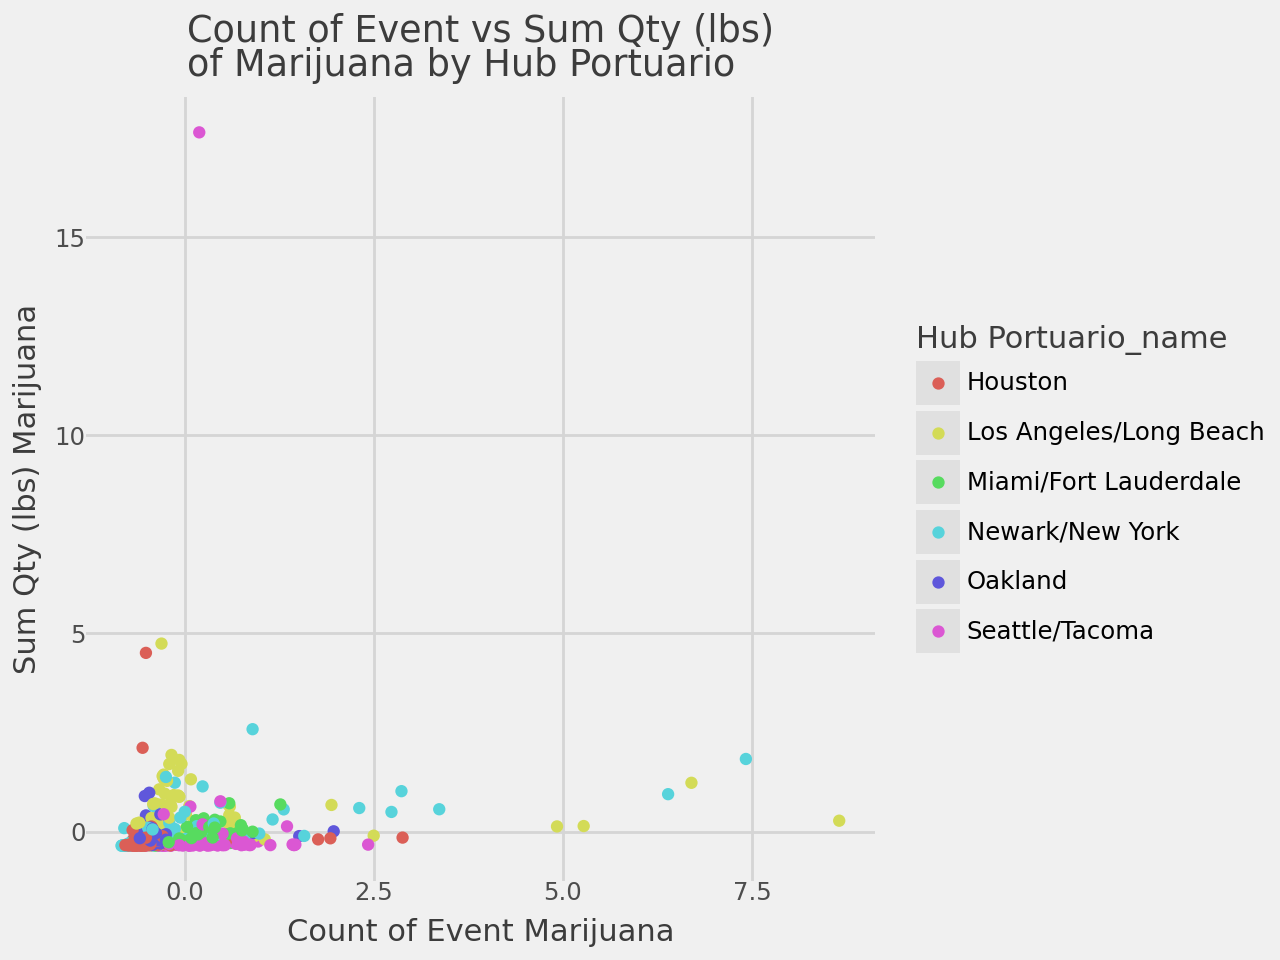
\includegraphics[width=\textwidth]{graph_ratios_3.png}
		\end{figure}
	
		\begin{figure}[H]
			\caption{\label{graph_ratios_4} Relación entre la cantidad de otras drogas incautadas y el número de redadas por puerto}
			\centering
			\hspace*{1cm}
			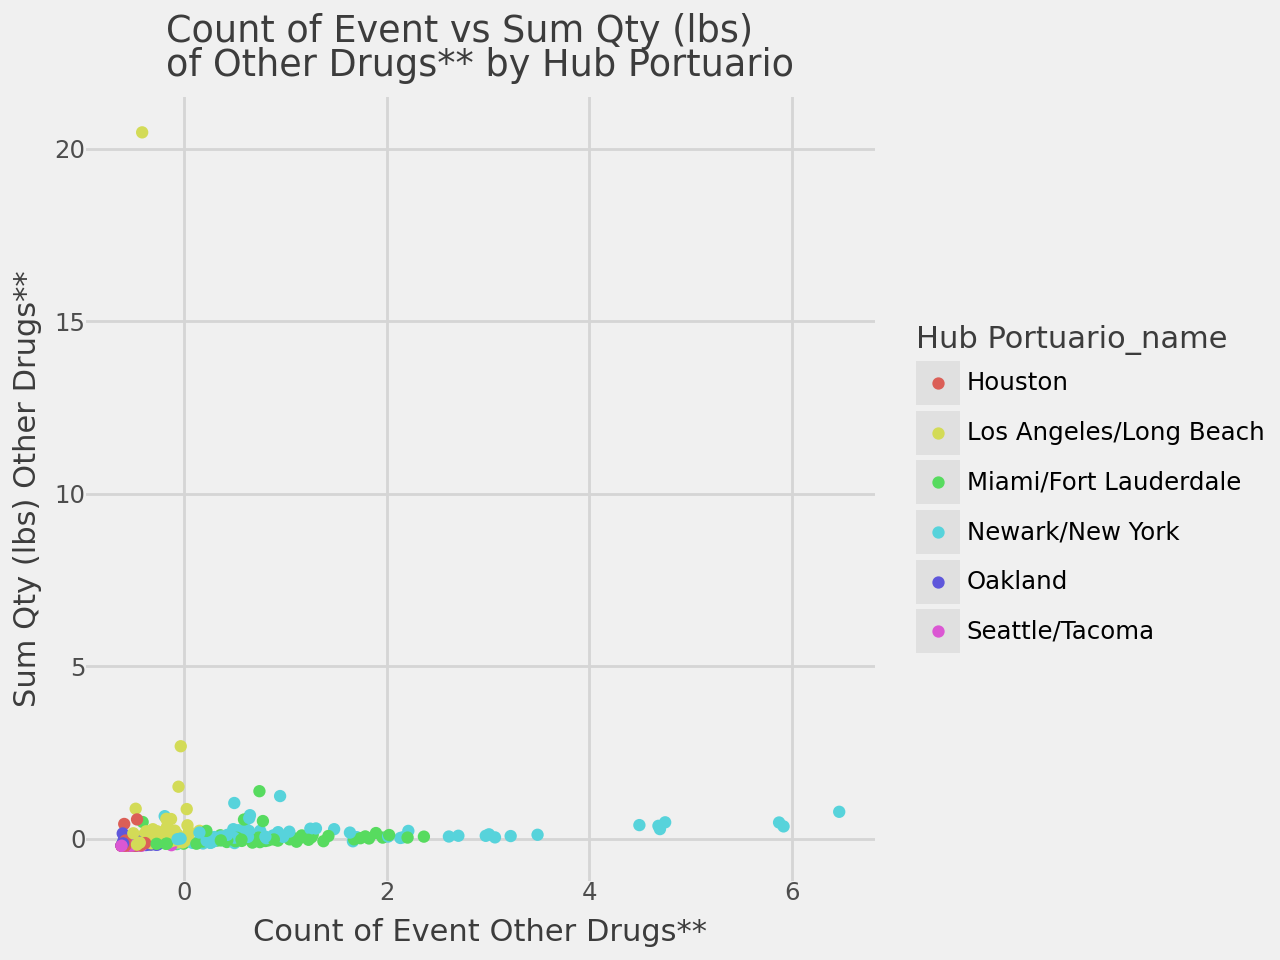
\includegraphics[width=\textwidth]{graph_ratios_4.png}
		\end{figure}
		
		% Incluir cálculo "Ratio_"
		% Cociente entre count event de tipo de drogas:
		$$
		Ratio\; of\; Drug\; Type = \frac{Sum\; Qty_i}{Count\; of\; Event_i}
		$$
		%
		Donde $i$ es cada tipo de droga.
		
		%Visualización en un mapa de Max Ratios:
		A continuación se muestran algunas visualizaciones para cada variable del tipo "Ratio" para cada tipo de droga en cada puerto:
		
		\begin{figure}[H]
			\caption{\label{map_bubble_5} Principales redadas por tipo de droga en cada puerto}
			\centering
			\hspace*{1cm}
			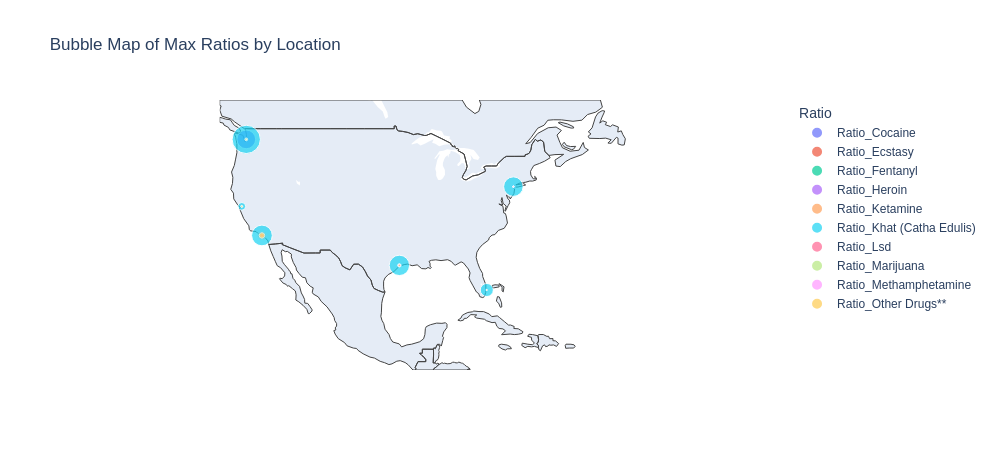
\includegraphics[width=\textwidth]{map_bubble_5.png}
		\end{figure}
		
		En todos los puertos se muestra que las redadas con mayor cantidad de droga incautada pertenecen a "Khat" debido a su poca implantación o dificultad para dar con ella. Véase la figura \ref{map_bubble_5}. Sin embargo, este tipo de drogas con pocos datos sobre ellas genera una cierta niebla e impresión distorsionada sobre grandes redadas.
		
		
		Como se mencionó en uno de los párrafos anteriores, con estas nuevas variables se buscaba ver a primera vista qué tipo de incautaciones se llevaban de forma regular para cada hub portuario. Por ejemplo, para los casos de incautaciones de cocaína, los puertos de Newark y de Miami eran constantes las redadas con importantes cantidades incautadas. Por otro lado, en Seattle/Tacoma se encontraron picos de incautación (similar a una delta) en algún mes concreto.
		
		% Incluir gráficas del Ratio Variables:
		Para el cálculo de las variables de ratio, se barajó realizar el cálculo a partir de los datos normalizados. Sin embargo, a la vista de resultados contradictorios, se decidió finalmente realizarlo sobre los datos brutos. Una de las contraindicaciones que surgía de esta última forma de calcularlo era la aparición de indeterminaciones del tipo 0/0 fruto de observaciones con missing values. Dado que los missing values correspondían a meses estimados sin redadas y, por lo tanto, sin incautaciones, y que el resto de valores eran forzosamente enteros positivos, el valor del ratio debía ser definitivamente, entero positivo, estrictamente mayor que cero. Estas aseveraciones permitieron, sin lugar a dudas, imputar los ratios en los casos de missing values a cero. Su sentido dentro del contexto de los datos de esa variable es que el cero es el mínimo valor para esa variable y que ninguna redada realizada podía alcanzar ese mínimo. Por su parte, el descarte de realizar el cálculo a partir de los datos normalizados era la paradoja resultante de obtener un ratio negativo (por debajo de la media) en el caso de tener una cantidad incautada elevada (valor positivo por encima de la media, numerador del cociente) frente un número bajo de redadas (valor negativo por debajo de la media, denominador del cociente) que, en relación con el resto de ratios, debería estar en el extremo positivo de la distribución. Finalmente, al igual que el resto de variables, antes de ser integradas en el dataset fueron estandarizadas mediante StandardScaler() implementado en el Pipeline de scikit-learn.
		
		% Suavizados de señales originales.
		% Derivadas sobre suavizados.
		También se estimó realizar un modelo basado en la comparación de tendencias entre variables de entrada (relacionadas con la gestión de los contenedores) y si el volumen de carga en un puerto mantiene alguna relación con la variación en la cantidad de droga total incautada. En este caso, fueron otras prioridades y ciertas restricciones de tiempo las que dejaron de lado este acercamiento al problema que hubiese sido, sin duda alguna, muy interesante de plantear. En todo caso, para lograr intuir la tendencia de señales temporales con mucho ruido habría que haber aplicado un filtro que suavizase la señal original y después derivar.
		
		%¿Por qué no se suman las cantidades de droga incautada?
		Pese a que hay elementos interesantes en favor de ello: la cantidad en kilogramos incautada de un tipo de droga A frente a otro tipo B no sería determinante a la hora de realizar un análisis y que podría inducir a error, quizá si lo fuese su equivalente en valor monetario -pero inviable en términos prácticos-.
		
	\subsection{Estrategia de división de datos}
	% Train-Test Split, Validación Cruzada, GridSearch para estimación de hiperparámetros.
	Para garantizar la correcta evaluación del rendimiento de los modelos desarrollados en este trabajo, resultó esencial definir una estrategia de división de datos. Con independencia del tipo de problema que se abordase, se consideró dejar como conjunto de datos libres de ser entrenados a todos aquellos con fechas más recientes a su captura (siendo la mayoría de ellos pertenecientes al año 2024). El resto de datos fueron usados para entrenar los distintos modelos junto con la evaluación y optimización de hiperparámetros para mejorar la precisión del modelo. La librería scikit-learn permite realizar tanto la división del conjunto de datos con train test split como la estimación de los hiperparámetros con GridSearchCV, entre otros.

\newpage
\section{\label{Diseño}Diseño del Modelo}
En esta sección se muestran los algoritmos y técnicas que se han utilizado para llevar a buen puerto el estudio en este proyecto. El objetivo de este trabajo se centra en intentar averiguar tendencias o patrones que relacionen el volumen de cargamento movido en contenedores gestionados por puertos con la cantidad de droga incautada. Así como para algún caso concreto, intentar hallar la relación temporal entre los mismos.

	\subsection{Algoritmos y técnicas de Machine Learning utilizados}

	% Hiperparámetros y técnicas de optimización.
	
	Como se vio en la sección \ref{motivacion}, hubo ciertas dificultades a la hora de plantear el target y, en definitiva, lo que quiere predecir el modelo. Se han desarrollado dos pequeños modelos al respecto: uno para predecir la cantidad incautada por redada en Newark (Estados de Nueva Jersey y Nueva York) y otro sobre la cantidad de redadas con éxito(*) en Port Everglades (Área Metropolitana Miami-Fort Lauderdale).
	
	\subsubsection{Implementación del algoritmo de clustering para detectar hubs portuarios}
	% Ver en colab
	
	% Detección de hubs portuarios: una primera incursión en modelos de Machine Learning.
	% No todos los puertos, a pesar de su volumen, tenían un emparejamiento claro con la agencia aduanera.
	
	
	\subsubsection{Implementación del algoritmo de Prophet para el análisis de series temporales}
	Algunos de los motivos que me llevó a plantear un modelo que ajustase series temporales fueron los resultados arrojados para incautaciones de drogas en el puerto de Fort Lauderdale. A continuación se muestran tres casos en los que se comparan las tendencias de importaciones (de contenedores con cargamento) junto con redadas de cocaína, marihuana y otras drogas. Fíjense que la distribución de los datos está ajustada a un escalado min-max (entre 0 y 1.00) y en las tendencias que tienen. Esto último abrió la posibilidad de orientar el trabajo a una aproximación de tendencias (derivadas de funciones suavizadas con filtros de bajas frecuencias) \ref{trabajo futuro}.
	
	\begin{figure}[H]
		\caption{\label{miami_ts_1} Serie Temporal en Puerto Fort Lauderdale con redadas de cocaína}
		\centering
		\hspace*{1cm}
		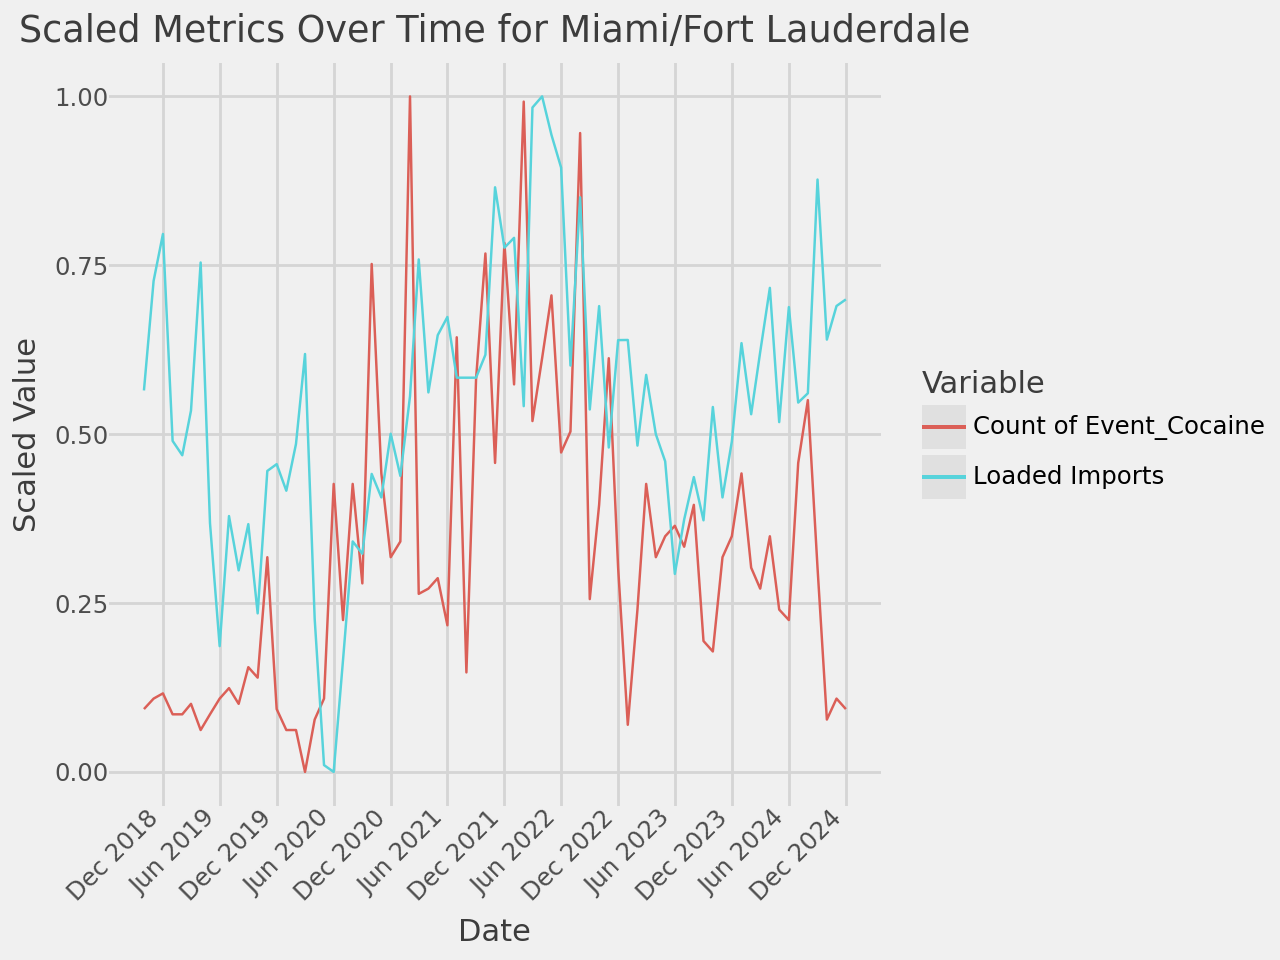
\includegraphics[width=\textwidth]{miami_ts_1.png}
	\end{figure}

	\begin{figure}[H]
		\caption{\label{miami_ts_2} Serie Temporal en Puerto Fort Lauderdale con redadas de otras drogas}
		\centering
		\hspace*{1cm}
		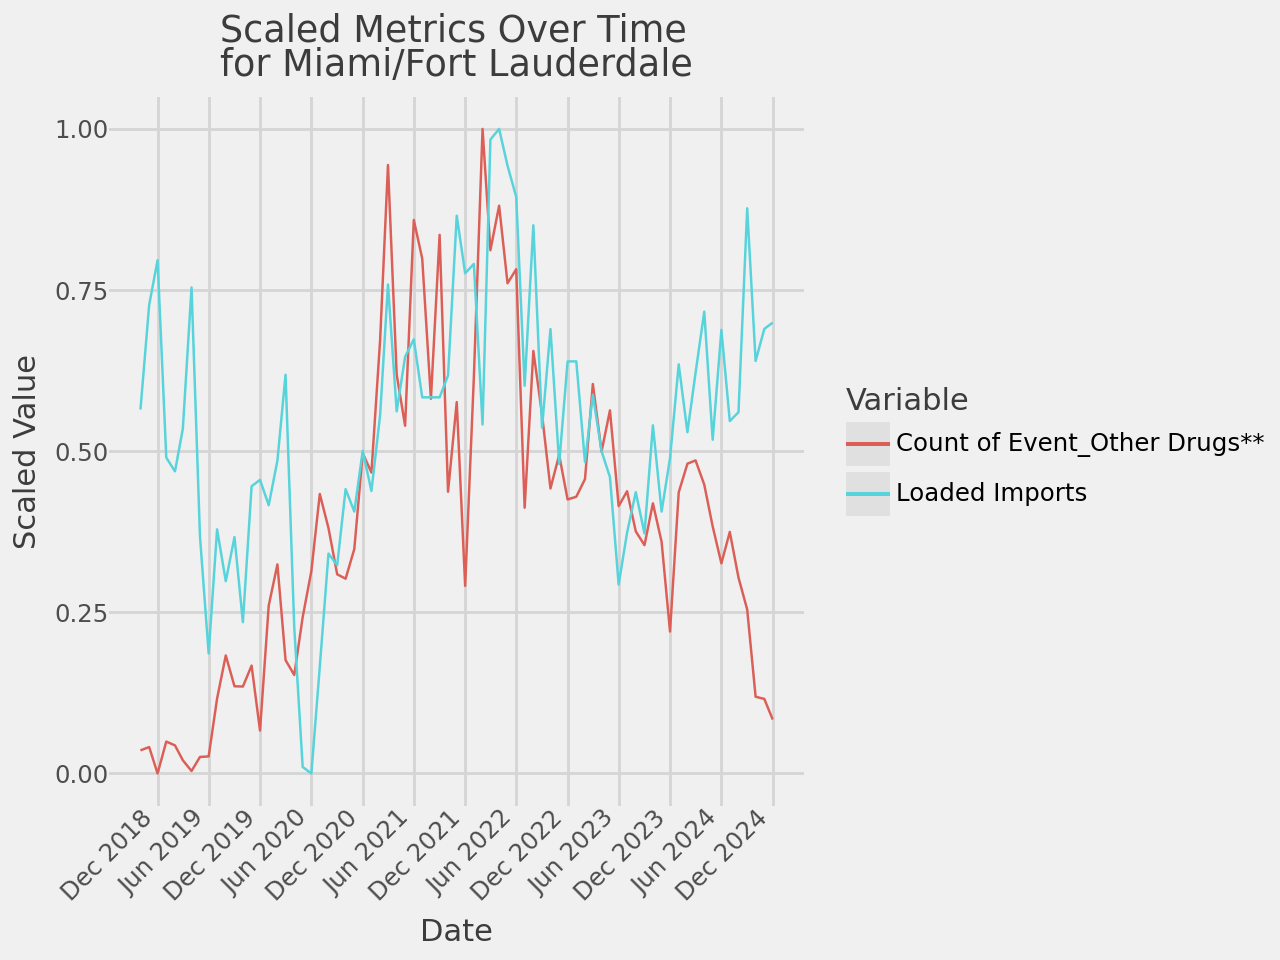
\includegraphics[width=\textwidth]{miami_ts_2.png}
	\end{figure}

	También en las secciones \ref{interpretacion} y \ref{trabajo futuro} se detallan los porqués de ciertos cambios de tendencia. Especialmente en el caso de \ref{miami_ts_2}, o por qué en la figura \ref{miami_ts_3} hay un lag entre las redadas de marihuana y el cargamento importado.
	
	\begin{figure}[H]
		\caption{\label{miami_ts_3} Serie Temporal en Puerto Fort Lauderdale con redadas de Marihuana}
		\centering
		\hspace*{1cm}
		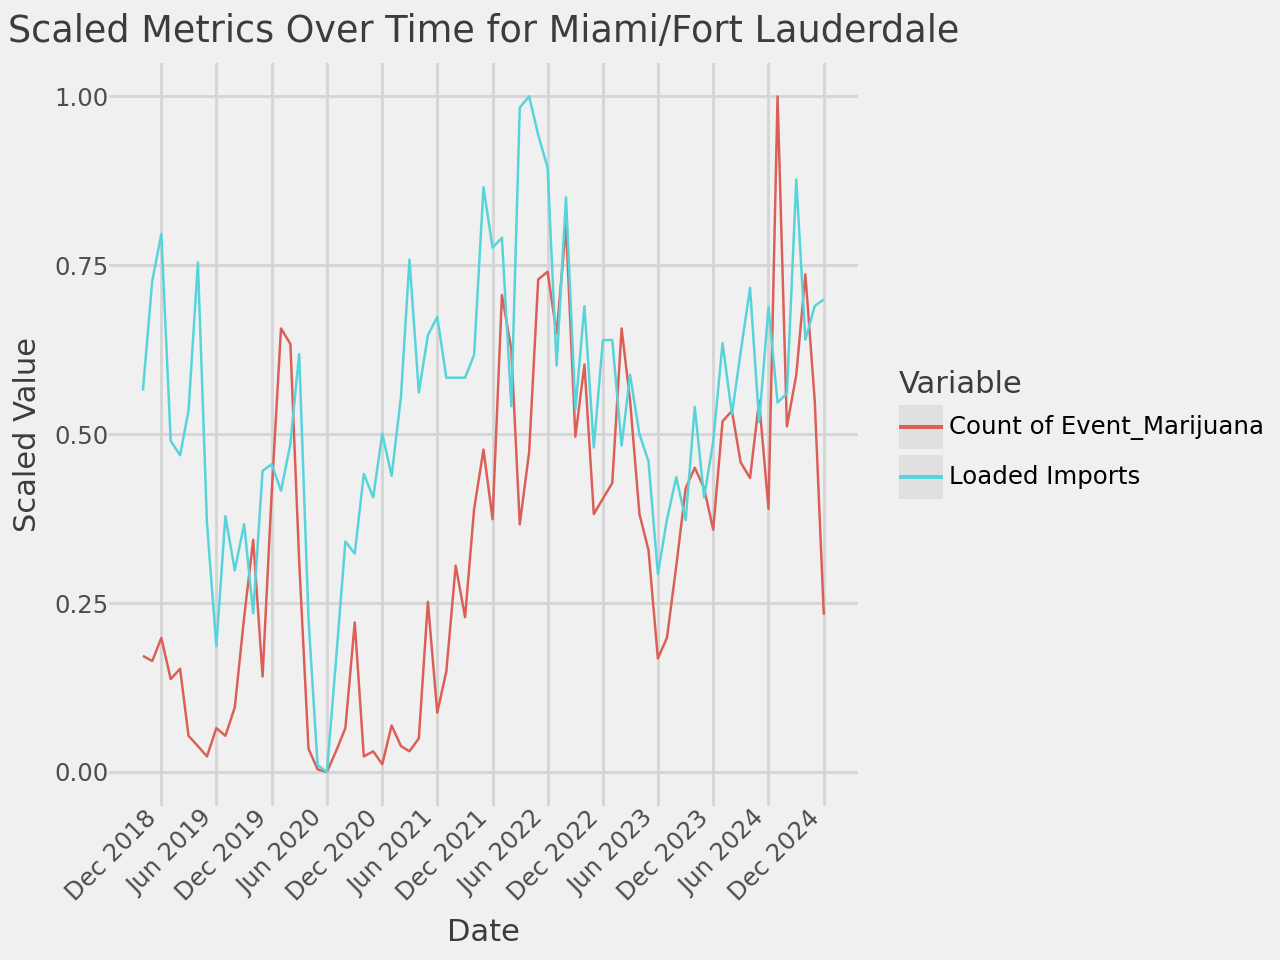
\includegraphics[width=\textwidth]{miami_ts_3.png}
	\end{figure}
	
	% Implementacion del modelo de serie temporal para Miami
	
	
	\subsubsection{Implementación de la matriz de ajuste hiperparámetros para los distintos algoritmos de regresión}
	% Copiar código de GridSearchCV
	

	\subsection{Implementación Práctica del Modelo}
 	- Descripción de las tareas realizadas para implementar el proyecto.
 	- Se destacan las principales actividades y decisiones.
 	- Fases de desarrollo del proyecto.
 	- Diagrama de Gantt con las tareas realizadas.
 	
 	% Modelo para el puerto de Nueva York
 	
 	% Modelo para Miami/Fort Lauderdale

	% Modelo para ajuste de una serie temporal

	\subsection{Evaluación del rendimiento}
	% Métrica utilizadas.
	% Comparaciones con alternativas.
	\begin{table}
	\caption{\label{tabla}}
		\centering
		\begin{tabular}{|c|c|c|c|c|c|c|}
			\hline
			Regressor &	mse\_train &	mse\_CV\_train &	mse\_validation &	mse\_test &	r2\_train &	r2\_test \\
			\hline
			GradientBoostRegressor &	0.131800 &	0.660717 &	-5.208851 &	0.262034 &	0.635442 &	-1.381853 \\
			baggingRegressor &	0.365540 &	0.322685 &	-5.609068 &	0.353780 &	-0.011080 &	-2.215812 \\
			AdaBoostRegressor &	0.058360 &	0.839348 &	-5.939976 &	0.277698 &	0.838576 &	-1.524235 \\
			LinearRegressor &	0.173767 &	0.530510 &	-6.821326 &	0.151522 &	0.519362 &	-0.377315 \\
			\hline
		\end{tabular}
	\end{table}

\newpage
\section{\label{interpretacion}Interpretación de los resultados}
Ninguno de los modelos fue capaz de predecir el comportamiento a futuro (obsérvese la columna de la métrica de r2 para el conjunto de test).

	\subsection{Visualización de resultados}
	
	
	\subsection{Sesgos y limitaciones}

\newpage
\section{\label{trabajo futuro}Conclusiones y trabajo futuro}

	\subsection{Hallazgos relevantes}
	
	\subsection{Aplicabilidad del modelo en entornos reales}
	
	\subsection{Limitaciones del trabajo}
	
	\subsection{Líneas de investigación futuras}

\newpage
\section{Bibliografía}
Pilgrim, G., E. Guidetti and A. Mourougane (2024), “An ocean of data: The potential of data on vessel traffic”, OECD Statistics Working Papers, No. 2024/02, OECD Publishing, Paris, https://doi.org/10.1787/34b7a926-en. 
https://www.portoflosangeles.org/business/statistics/container-statistics/historical-teu-statistics-2020
https://www.cbp.gov/
https://www.cbp.gov/document/stats/nationwide-drug-seizures
https://www.cbp.gov/document/stats/amo-drug-seizures
https://www.portofsandiego.org/
https://www.nwseaportalliance.com/about-us/cargo-statistics
https://plotnine.org/
https://docs.profiling.ydata.ai/latest/
https://plotly.com/python/
https://www.miamidade.gov/portmiami/cargo.asp
https://southfloridacontainer.com/
http://pomtoc.com/
https://www.seaboardmarine.com/
https://assets.simpleviewinc.com/simpleview/image/upload/v1/clients/porteverglades/January\_Monthly\_Loaded\_TEUs\_02\_13\_2025\_9e6f70c1-032a-4bbc-8f69-2d027dcfa394.pdf
https://assets.simpleviewinc.com/simpleview/image/upload/v1/clients/porteverglades/FY2023\_September\_TEUS\_Loaded\_by\_Month\_7065b619-cddd-4b97-a02c-8c247c743ac0.pdf
https://assets.simpleviewinc.com/simpleview/image/upload/v1/clients/porteverglades/August\_TEUS\_Loaded\_by\_Month\_Fiscal\_2020\_Calander\_2020\_9439e3f7-7154-4030-a9b8-9ec592a57fde.pdf
https://assets.simpleviewinc.com/simpleview/image/upload/v1/clients/porteverglades/Preliminary\_Waterborne\_Commerce\_Chart\_2024\_\_1a6b16e6-94b2-46ac-89e7-d7080779f346.pdf
https://www.panynj.gov/port/en/our-port/facts-and-figures.html
https://arxiv.org/abs/1208.5801
https://towardsdatascience.com/time-series-from-scratch-decomposing-time-series-data-7b7ad0c30fe7/\#:~:text=a\%20single\%20season.-,Multiplicative\%20trend\%20and\%20additive\%20seasonality,of\%20seasonal\%20periods\%20over\%20time.\&text=You\%20can\%20see\%20how\%20the\%20trend\%20is\%20slightly\%20curved
https://www.wired.com/2012/04/april-26-1956-the-container-ships-maiden-voyage/
8878396-2.pdf
citar a [Source: adapted from D.M. Bernhofen, Z. El-Sahli and R. Kneller (2013) Estimating the Effects of the Container Revolution on World Trade, Lund University, Department of Economics, Working Paper 2013:4.]s

Puertos en el análisis: Los Angeles, Long Beach, Seattle, Tacoma, Everglades-Fort Lauderdale, Houston, Newark-New York, Oakland.

\newpage
\section{Glosario}
\begin{description}
	\item CBP: US Customs and Border Protection. Oficina de Aduanas y Protección Fronteriza de los Estados Unidos (Agencia del gobierno federal).
	\item Field Office: Oficina Regional de la Agencia Federal de Control de Fronteras y Aduanas (CBP en sus siglas originales).
	\item MNAR: Missing Not At Random.
	\item TEU (Twenty-Foot Equivalent Unit): unidad de medida equivalente a un contenedor (caja de metal) con medidas estándares (ISO 668). Facilidad de transferencia intermodal. Sus dimensiones son: 8'6" de alto x 8" de ancho x 20-ft de pie.
	\item señal AIS:
	\item NOAA: Agencia de meteorología del gobierno de Estados Unidos (National Oceanic and Atmospheroc Agency, por sus siglas en inglés)
	\item SFBA: Área Metropolitana de la Bahía de San Francisco (incluye el puerto de Oakland)
	\item GLA: Área Metropolitana del Gran Los Ángeles
\end{description}

\newpage
\section{Anexos}
Otras imágenes:

\begin{figure}[H]
	\caption{\label{timeseries_3} Serie temporal sobre redadas por tipo de droga en Newark}
	\centering
	\hspace*{1cm}
	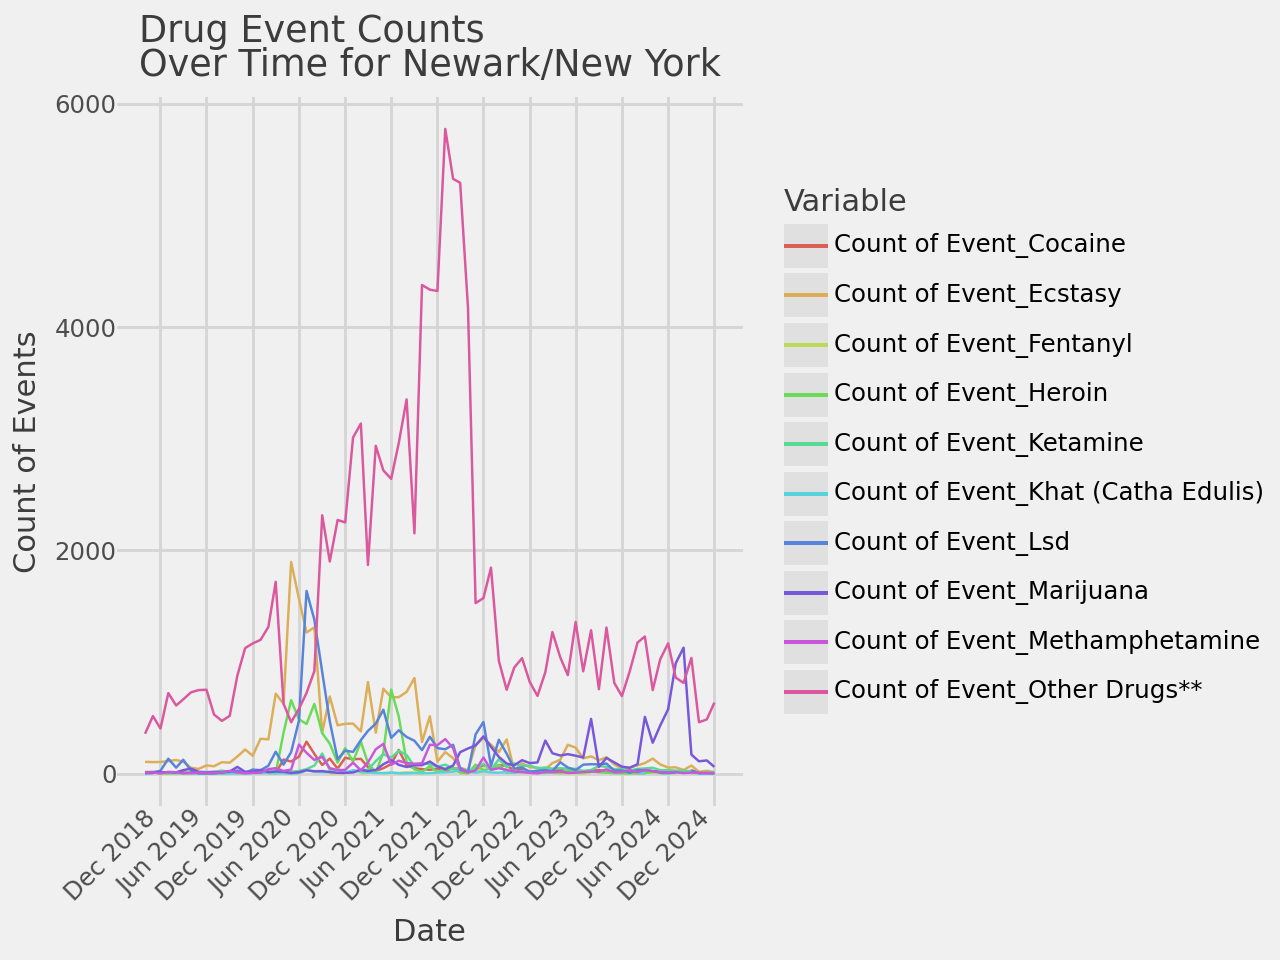
\includegraphics[width=\textwidth]{timeseries_3.png}
\end{figure}

\begin{figure}[H]
	\caption{\label{timeseries_4} Serie temporal sobre redadas por tipo de droga en Seattle}
	\centering
	\hspace*{1cm}
	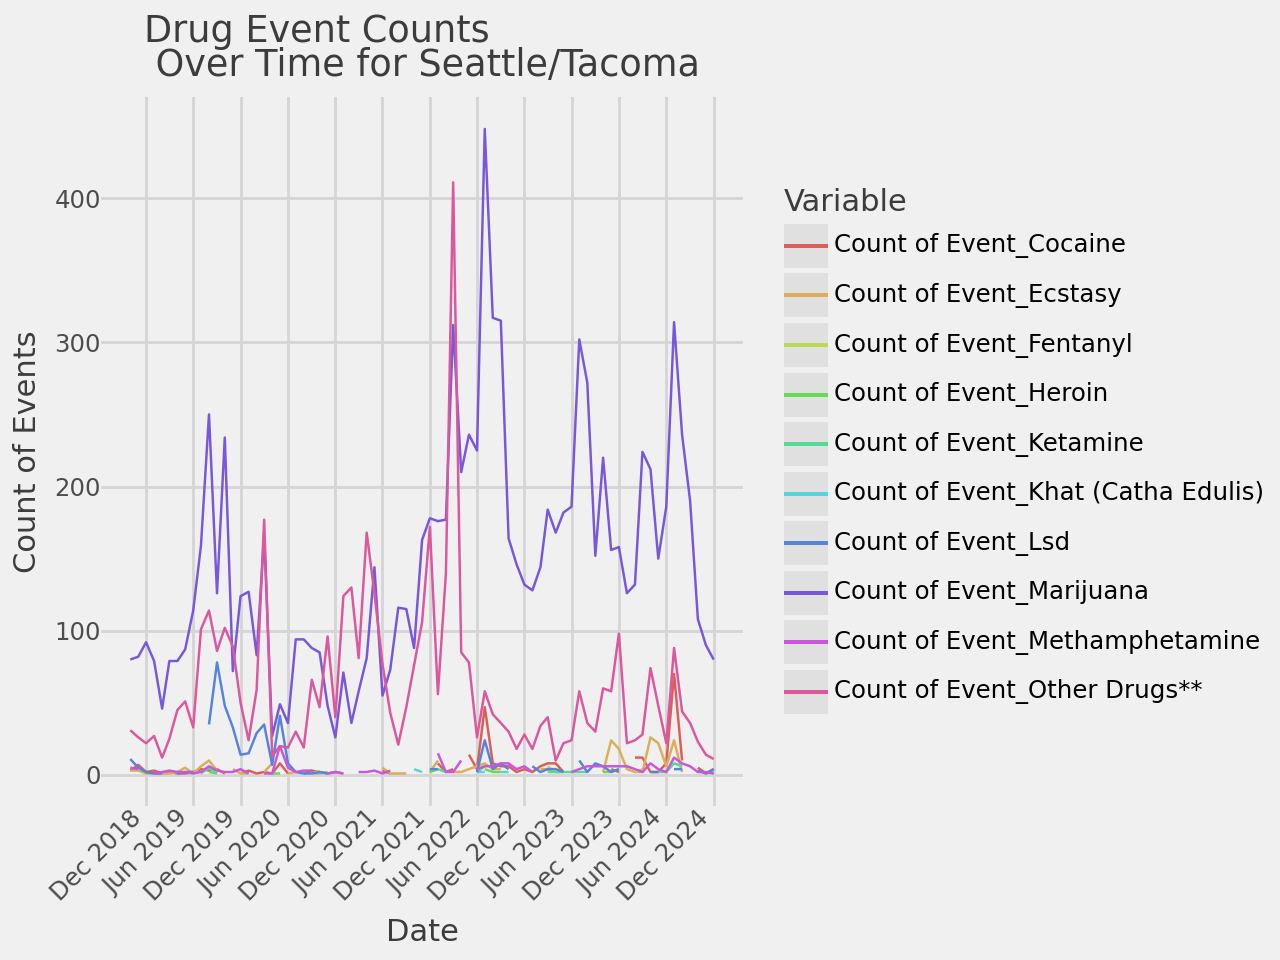
\includegraphics[width=\textwidth]{timeseries_4.png}
\end{figure}

\begin{figure}[H]
	\caption{\label{timeseries_5} Serie temporal sobre redadas por tipo de droga en Los Angeles}
	\centering
	\hspace*{1cm}
	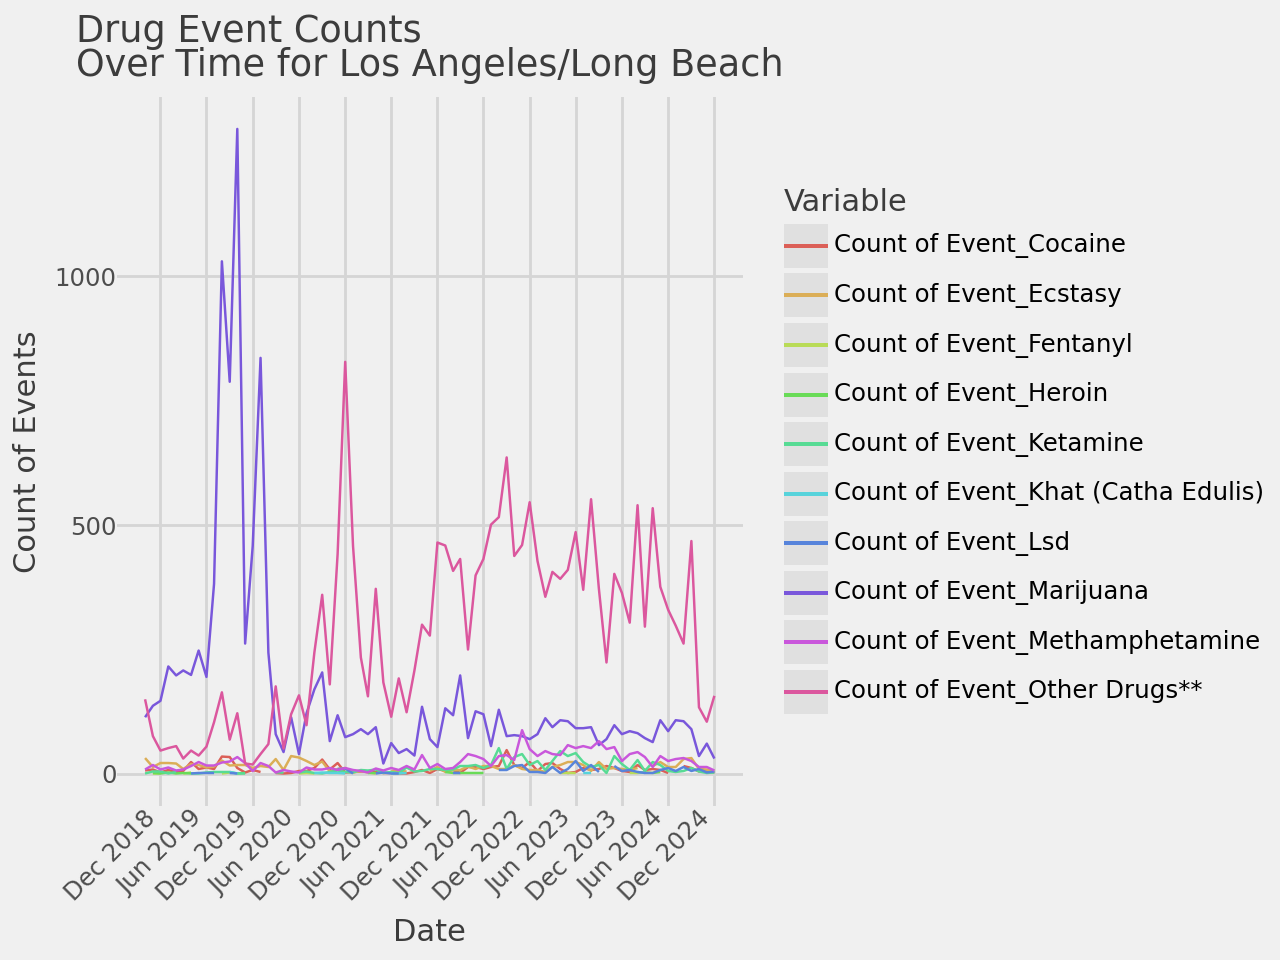
\includegraphics[width=\textwidth]{timeseries_5.png}
\end{figure}

\begin{figure}[H]
	\caption{\label{timeseries_5} Serie temporal sobre redadas por tipo de droga en Los Angeles}
	\centering
	\hspace*{1cm}
	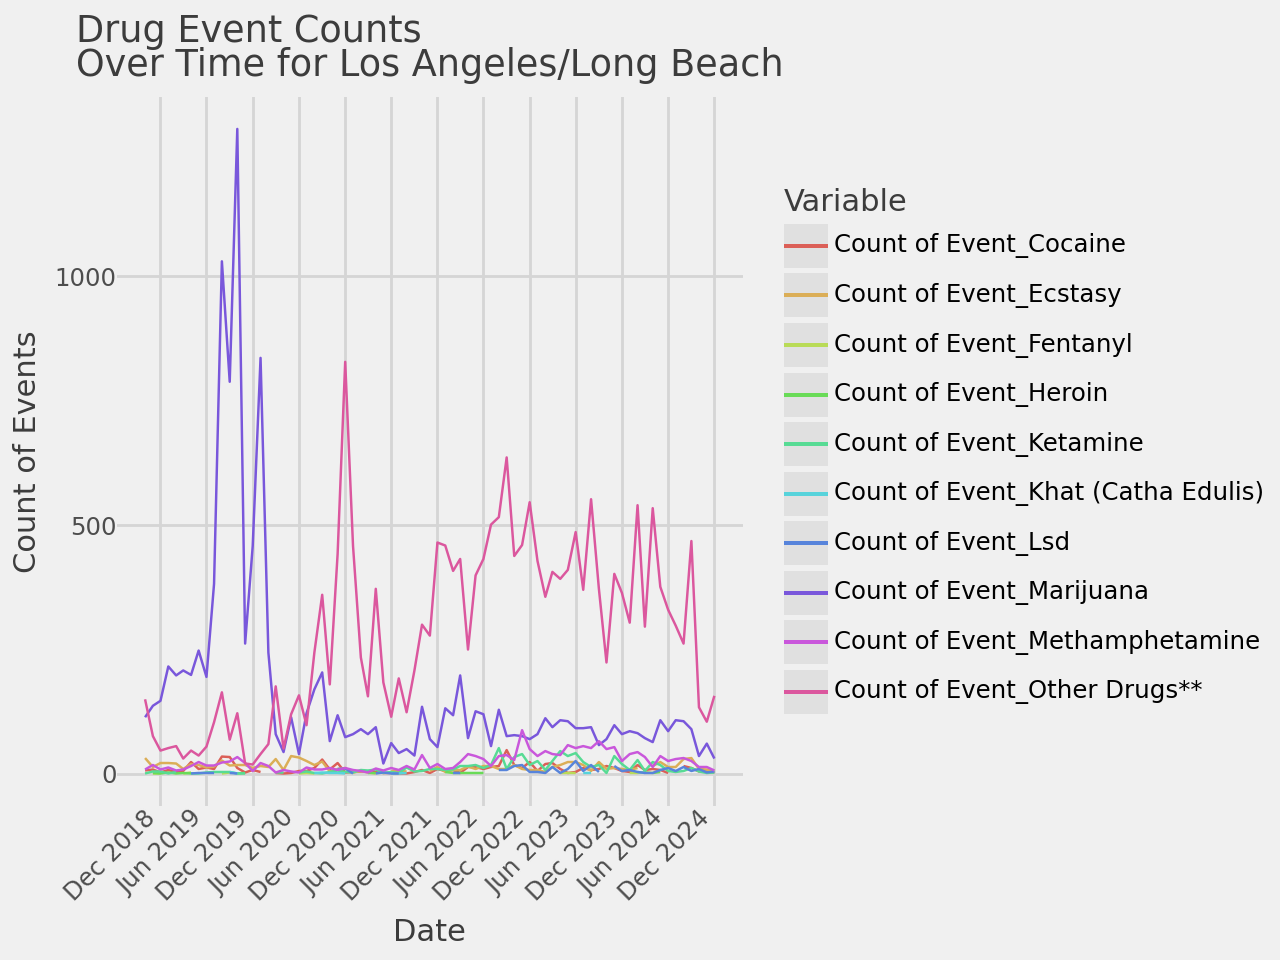
\includegraphics[width=\textwidth]{timeseries_5.png}
\end{figure}

\begin{figure}[H]
	\caption{\label{hist_4} Distribución de redadas por mes en Newark}
	\centering
	\hspace*{1cm}
	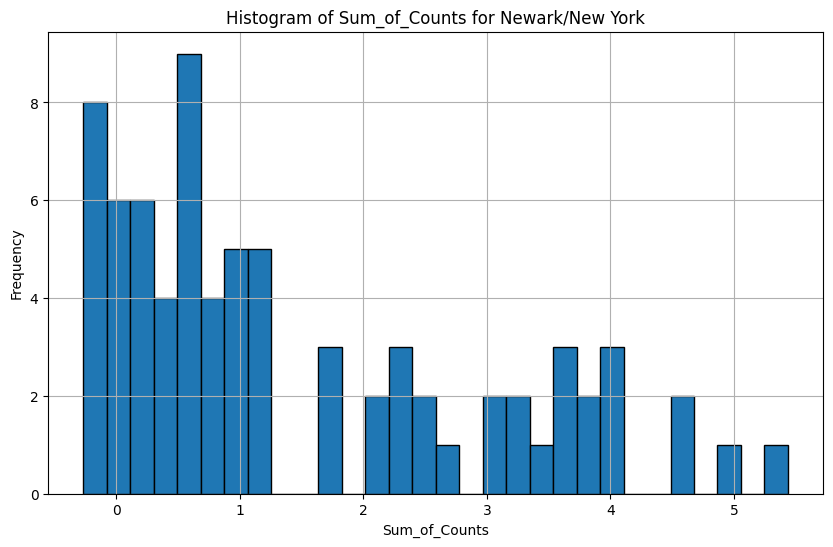
\includegraphics[width=\textwidth]{hist_4.png}
\end{figure}

\begin{figure}[H]
 	\caption{\label{hist_5} Distribución de redadas por mes en Newark}
 	\centering
 	\hspace*{1cm}
 	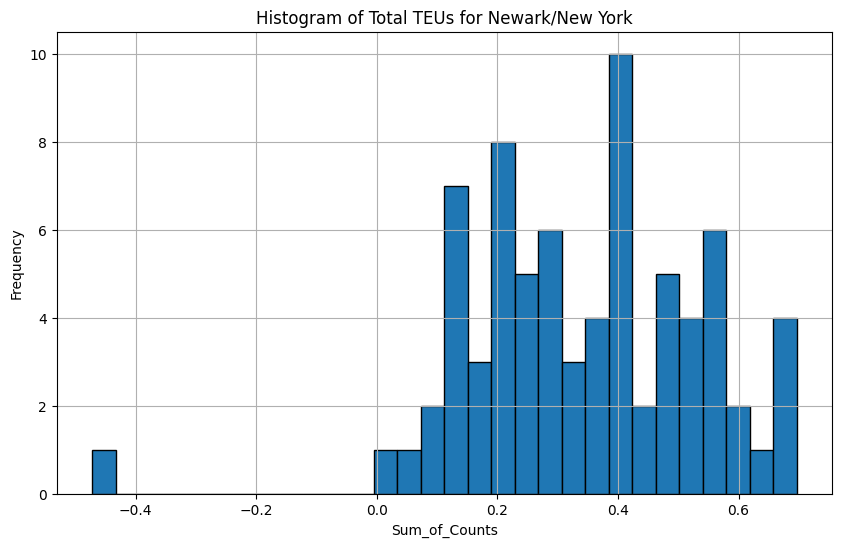
\includegraphics[width=\textwidth]{hist_5.png}
\end{figure}

\end{document}


%Pre procesamiento de los datos

%EDA, Limpieza, tratamiento de outliers.

 